%%%%%%%%%%%%%%%%%%%%%%%%%%%%%%%%%%%%%%%%%%%%%%%%%%
%% Bachelor's & Master's Thesis Template        %%
%% Copyleft by Dawid Weiss & Marta Szachniuk    %%
%% Faculty of Computing and Telecommunication   %%
%% Poznan University of Technology, 2020        %%
%%%%%%%%%%%%%%%%%%%%%%%%%%%%%%%%%%%%%%%%%%%%%%%%%%


% Szkielet dla pracy licencjackiej pisanej w języku polskim.

\documentclass[polish,bachelor,a4paper,oneside]{ppfcmthesis}


\usepackage[utf8]{inputenc}
\usepackage[OT4]{fontenc}
\usepackage{listings}
%--------------------------------------
% Strona tytułowa
%--------------------------------------

% Autorzy pracy, jeśli jest ich więcej niż jeden
% wstaw między nimi separator \and
\author{%
   Zofia Fraś \album{136703} \and 
   Marcin Jachymski \album{136718} \and
   Krzysztof Sobkowiak \album{136799} \and
   Agnieszka Szuflak \album{136812}
   }
\authortitle{}                                % Do not change.

\title{Komputerowy system wspomagający diagnostykę i~raportowanie w~gabinetach stomatologicznych}

% Your supervisor comes here.
\ppsupervisor{~dr hab.~inż.~Paweł Śniatała prof. PP} 

% Year of final submission (not graduation!)
\ppyear{2020}         


\makeatletter

\newcommand\cfbox[3][lbrt]{%
  \begingroup
  \leavevmode
  \setbox\@tempboxa\hbox{%
    \color@begingroup
      \kern\fboxsep{#3}\kern\fboxsep
    \color@endgroup
  }%
  \@tempdima\fboxrule
  \advance\@tempdima\fboxsep
  \advance\@tempdima\dp\@tempboxa
  \hbox{%
    \hskip-.5\fboxrule
    \lower\@tempdima\hbox{%
      \vbox{%
        \in@{t}{#1}%
        \ifin@
            {\color{#2}%
            \hrule\@height\fboxrule
            }%
        \fi
        \hbox{%
          \in@{l}{#1}%
          \ifin@
            {\color{#2}%
            \vrule\@width\fboxrule
            }%
          \fi
          \vbox{%
            \vskip\fboxsep
            \box\@tempboxa
            \vskip\fboxsep}%
          \in@{r}{#1}%
          \ifin@
            {\color{#2}%
            \vrule\@width\fboxrule
            }%
          \fi
        }%
        \in@{b}{#1}%
        \ifin@
          {\color{#2}%
          \hrule\@height\fboxrule
          }%
        \fi
      }%
    }%
    \hskip-.5\fboxrule
  }%
  \endgroup
}

\makeatother


\begin{document}

% Front matter starts here
\frontmatter\pagestyle{empty}%
\maketitle\cleardoublepage%

%--------------------------------------
% Miejsce na kartę pracy dyplomowej
%--------------------------------------

\thispagestyle{empty}\vspace*{\fill}%
\begin{center}Tutaj będzie karta pracy dyplomowej;\\oryginał wstawiamy do wersji dla archiwum PP, w~pozostałych kopiach wstawiamy ksero.

Czy ten tekst usunąć?
\end{center}%
\vfill\cleardoublepage%

%--------------------------------------
% Streszczenie
%--------------------------------------

%\documentclass[../main.tex]{subfiles} 
\chapter{Streszczenie}
%\begin{document}

Nie wiem czy to pisać. Napisał bym to samo co we wstępie + kawałem z podsumowania

\vspace*{\fill \textbf{\textit{Słowa kluczowe---}} System oznaczania zębów, Rozpoznawanie obrazów, Asystent głosowy} % Moves keywords to the bottom of the page


%\biblio % Needed for referencing to working when compiling individual subfiles - Do not remove

%\end{document}

\pagenumbering{gobble}
\clearpage

%--------------------------------------
% Spis treści
%--------------------------------------

\tableofcontents* 
\pagenumbering{gobble}
\cleardoublepage % Zaczynamy od nieparzystej strony

%--------------------------------------
% Spis rysunków
%--------------------------------------

\listoffigures* 
\pagenumbering{gobble}
\cleardoublepage % Zaczynamy od nieparzystej strony

%--------------------------------------
% Spis tablic
%--------------------------------------

\listoftables*
\pagenumbering{gobble}
\cleardoublepage % Zaczynamy od nieparzystej strony
%--------------------------------------
% Rozdziały
%--------------------------------------

%Najwygodniej jeśli każdy rozdział znajduje się w oddzielnym pliku
\mainmatter%

\chapter{Wstęp}


Gabinety dentystyczne od wielu lat korzystają z procesu informatyzacji. Pełna obsługa klienta, katalogi, zdjęcia - to wszystko zostało przeniesione z dokumentacji papierowej do cyfrowego świata. Zmiana ta dotknęła jednakże bardziej pracowników administracyjnych czy asystentów stomatologów, niż samych lekarzy\cite{dentalSurvay}. Lekarze nadal muszą wykonywać wiele czynności ręcznie takich jak uzupełnianie dokumentacji po wizycie czy wykrywanie i~opisywanie schorzeń. Obecny poziom technologii pozwala na znaczne zwiększenie stopnia automatyzacji i~liczby usprawnień przy pracy w~klinikach dentystycznych.

Celem pracy jest zaprojektowanie dwóch modułów ułatwiających pracę stomatologom. Pierwszy moduł to nowoczesny diagram zębowy posiadający możliwość wprowadzania danych komendami głosowymi. Jest to propozycja rozwiązania problemu wypełniania dokumentacji po wizycie. Dzięki interfejsowi głosowemu lekarz może uzupełniać diagram zębowy w~czasie pracy z klientem. Drugim modułem jest detektor wady zgryzu [tor odwodzenia żuchwy]. Na podstawie prostego filmiku otwierania żuchwy przez pacjenta, moduł jest wstanie obliczyć nieprawidłowość w~torze odwodzenia żuchwy i~opracować raport. Automatyzacja tego procesu pozwoli na uproszczenie badania co przełoży się na większą ilość osób badanych. Wymaga również mniej czasu od stomatologa.

Implementacja modułów pozwala w~prosty sposób dołączyć je do istniejących systemów i~programów dentystycznych. W~celu ułatwienia dostępu, każdy moduł będzie w~stanie działać samodzielnie jako aplikacja desktopowa. 

Ważną częścią pracy jest użyteczność projektu. Oznacza to, że implementacja projektu jest zgodna ze standardami medycznymi, które są naturalne dla pracy stomatologów. Część literatury będzie mieć w~związku z tym podłoże medyczne. Duża część podstaw teoretycznych będzie się skupiała na wyjaśnieniu podstaw terminologii stomatologicznej, tak aby łatwiej było zrozumieć niektóre decyzje architektoniczne. W~literaturze znajdą się również pozycje związane z zastosowanymi algorytmami oraz z użytymi technologiami.

Struktura pracy jest następująca. W~rozdziale drugim przedstawiono podstawy teoretyczne związane z powyżej opisaną literaturą. Rozdział trzeci jest poświęcony użytym technologiom. Opisy działania przedstawiają najważniejsze aspekty z uwagi na które dany framework, biblioteka czy program został wybrany do projektu. Rozdział ten pokazuje również niektóre funkcjonalności z bardziej niskopoziomowej strony. Następny rozdział czwarty przedstawia bardziej ogólną budową i~architekturę obydwu modułów. Opisuje również jak działa komunikacja i~przepływ danych. Rozdział piąty skupia się na pokazaniu aplikacji od strony użytkownika. Referuje możliwości aplikacji i~przypadki użycia. Na koniec opisuje proces testowania oraz trudności jakie wystąpiły przy tworzeniu programu. Ostatni rozdział szósty jest podsumowaniem całej pracy. Przedstawia rezultaty jakie udało się uzyskać, a~także wizję rozwoju aplikacji w~przyszłości.


\section{Struktura prac}
Praca od początku została określona jako dwa osobne moduły. W~związku z tym w~większości rozdziałów pracy obowiązuje podział na ,,System oznaczania zębów'' oraz ,,Rozpoznawanie wady zgryzu''. Obydwie części mają taki sam cel, który opisano wcześniej. Nad każdym modułem pracowały dwie osoby. Podział prac został określony i~zrealizowany w~sposób:
\subsection{System oznaczania zębów}
nie wiem czy bardziej czy mniej ogólnie, niech śniatała powie jak będzie sprawdzał


\textbf{Zofia Fraś}
\begin{itemize}
    \item moje pomysły:
    \item Budowa klienta
    \item Zaprojektowanie i ewaluacja projektu graficznego diagramu zębowego
    \item Stworzenie procesu asynchronicznej aktualizacji zmian dokonywanych przez interfejs głosowy
    \item Walidacje pól - jakoś ładniej
    \item Zadbanie o UX - to jakoś inaczej
    \item Stworzenie systemu obsługi diagramu zębowego
    \item Projekt i realizacja interfejsu graficznego aplikacji
    \item Cos o widoku formularza osobowego?
    \item Testy manualne 
\end{itemize}

\textbf{Krzysztof Sobkowiak}    
\begin{itemize}
    \item Budowa serwera
    \item Obsługa nierelacyjnej bazy danych i przetwarzanie danych w formacie JSON
    \item Komunikacja klient-serwer
    \item Interfejs głosowy, w tym połączenie z Google Speech Recognition API
    \item Stworzenie, obsługa i testowanie słowników interfejsu głosowego
    \item Algorytm klasyfikacji komend głosowych
    \item Proces wersjonowania
    \item Zarządzanie repozytorium projektu w serwisie GitHub
\end{itemize}

\subsection{Analiza odchylenia toru odwodzenia żuchwy}
\textbf{Marcin Jachymski}
\begin{itemize}
    \item Detekcja zębów
    \item Śledzenie ruchu zębów
\end{itemize}

\textbf{Agnieszka Szuflak}    
\begin{itemize}
    \item Interfejs użytkownika
    \item Obliczenie odległości i kątów
\end{itemize}

\section{Repozytoria}
Projekt została zrealizowana w~oparciu o~narzędzie kontroli wersji Git, a~publiczne repozytoria umieszczone w~serwisie GitHub:

\begin{itemize}
    \item Praca inżynierska:
    
    \url{}

    \item System oznaczania zębów:
    
    \url{https://github.com/kszysix/dental-data-procesing}
    
    \item Analiza odchylenia toru odwodzenia żuchwy:
    
    \url{}
\end{itemize}

\section{TODO}
Co trzeba zrobić i na co zwracać uwagę:
\begin{itemize}
\item "nie wiem o~czym pisać" / "nie wiem jak dużo pisać":
\begin{itemize}
    \item temat: na podstawie tytułu sekcji znajdź pojęcie informatyczne np. RESTapi, metody zapisu i kompresji obrazu, 
    \item znajdź tekst na legitnej stronce po angielsku
    \item znajdz coś naukowego co potwierdza mniej więcej tekst ze stronki
    \item dodaj cytowanie 
    \item przetłumacz tekst ze stronki (samemu!), dzięki czemu już nie robisz plagiatu bo piszesz swoimi słowami
    \item zalinkuj cytowanie w~pracy
    \item bonus: dodaj legitny obrazek razem ze źródłem.\cite{restapi}
\end{itemize}
    \item każda opinia powinna być potwierdzona odnośnikiem do strony/artykułu/pracy
    \item w~każdej sekcji a~najlepiej podsekcji powinny znaleźć się odnośniki do literatury
    \item spokojnie w~co drugiej podsekcji może być jakiś obrazek, najlepiej jakiś diagram pokazujący działanie. Przy czym źródło obrazka też powinno być w~miarę legitne
    \item warto rozpisywać się o~wszystkim - każdym szczególne np. w~jaki sposób jest coś wyśrodkowane na froncie czy jakich standardów używa biblioteka i opisać standard lub 
    \item Na koniec trzeba sprawdzić zasady opisane w~załączniku np. myślniki, miejsca cytowań, twarda spacja! 
    \item po ustawiać zdjęcia na koniec
    \item czy zamiast "wada zgryzu" powinno być "dewiacja zgryzu"
    \item np. Jakie zalety i wady posiada openCv? jakie są alternatywy? jak działa licencja?
    
Jaki format obrazu (czy typ danych) ma filmik i klatka? wady i zalety fomratu?

*wszędzie* :

jaka jest licencja?

jakie są alternatywy?

wady i  zalety

jakie są różnice między klasycznym użyciem a~użyciem w~aplikacji?

\end{itemize}
    


\chapter{Podstawy teoretyczne}

coś tutaj można napisać z~3-4 liniki wprowadzenia co to za rozdział, we wstępie to jest opisane
 
\section{System oznaczania zębów}

Istnieje wiele systemów służących do zapisywania stanu uzębienia pacjentów. Pomagają one w~przejrzysty sposób przechowywać dane, które mogą być przekazywane między pracownikami służby zdrowia wykorzystującymi różne programy oraz standardy. Nie wymagają wówczas skomplikowanej analizy - jednoznacznie i~w~prosty sposób przedstawiają wprowadzone wcześniej dane. Dodatkowo są~zrozumiałe i~przystępne dla pacjentów.

Każdy z~systemów wyróżnia zbiór reguł, według których zęby, z~rozróżnieniem na zęby mleczne oraz stałe, są kolejno nazywane. W~najbardziej popularnych systemach, które zostały przedstawione poniżej, zęby podzielone są na cztery podzbiory oznaczane jako: łuk górny prawy, łuk górny lewy, łuk dolny lewy oraz łuk dolny prawy. Schematy przedstawiają na planie krzyża uzębienie widziane z~perspektywy lekarza, a~nazwy dotyczą perspektywy pacjenta.

\subsection{Przegląd systemów}
\subsubsection{System łaciński}

\renewcommand*{\tablename}{Schemat}

System ten wykorzystuje w~nazewnictwie pierwsze litery łacińskich nazw zębów. Stąd w~każdej ćwiartce dwa siekacze oznaczane są literą \textit{I} - od słowa \textit{incisivi} - i~kolejno numerowane, kły literą \textit{C} - od słowa \textit{canini}, oznaczenie dwóch przedtrzonowców pochodzi od słowa \textit{premolares} - litera \textit{P} oraz trzech trzonowców od słowa \textit{molares} - litera \textit{M}. W~systemie łacińskim oprócz nazwy zęba, która powtarza się w~czterech podzbiorach, dodaje się także nazwę ćwiartki, do której ząb należy, definiując czy jest górna czy też dolna oraz czy lewa albo prawa.\\

\begin{table}[h t]
\centering
\begin{tabular}{c c c c c c c c c | c c c c c c c c c}
M\textsubscript{3} & M\textsubscript{2} & M\textsubscript{1} & P\textsubscript{2} & P\textsubscript{1} & C & I\textsubscript{2} & I\textsubscript{1} &&& I\textsubscript{1} & I\textsubscript{2} & C & P\textsubscript{1} & P\textsubscript{2} & M\textsubscript{1} & M\textsubscript{2} & M\textsubscript{3}
\\ [1ex] \hline \rule{0pt}{1.2\normalbaselineskip}
M\textsubscript{3} & M\textsubscript{2} & M\textsubscript{1} & P\textsubscript{2} & P\textsubscript{1} & C & I\textsubscript{2} & I\textsubscript{1} &&& I\textsubscript{1} & I\textsubscript{2} & C & P\textsubscript{1} & P\textsubscript{2} & M\textsubscript{1} & M\textsubscript{2} & M\textsubscript{3}
\end{tabular}
\caption{\label{tab:tab1} System łaciński: zęby stałe}
\end{table}

Opisane powyżej nazewnictwo dotyczy zębów stałych człowieka. Zęby mleczne oznacza się jednak analogicznie, zamieniając jedynie wielkie litery na małe - \textit{i}, \textit{c}, \textit{m} oraz opisując pięć zębów w~każdej ćwiartce - dwa siekacze, kieł oraz dwa zęby trzonowe.

\begin{table}[h t]
\centering
\begin{tabular}{c c c c c c | c c c c c c}
m\textsubscript{2} & m\textsubscript{1} & c & i\textsubscript{2} & i\textsubscript{1} &&& i\textsubscript{1} & i\textsubscript{2} & c & m\textsubscript{1} & m\textsubscript{2}
\\ [1ex] \hline \rule{0pt}{1.2\normalbaselineskip}
m\textsubscript{2} & m\textsubscript{1} & c & i\textsubscript{2} & i\textsubscript{1} &&& i\textsubscript{1} & i\textsubscript{2} & c & m\textsubscript{1} & m\textsubscript{2}
\end{tabular}
\caption{\label{tab:tab2} System łaciński: zęby mleczne}
\end{table}

\subsubsection{System Zsigmondy’ego}

System Zsigmondy'ego, podobnie jak system łaciński, definiuje taką samą nazwę dla odpowiadających sobie zębów w~kolejnych ćwiartkach i~dodaje do niej oznaczenie jednej z~czterech części. Zęby są tutaj numerowane od 1 do 8, zaczynając od siekaczy znajdujących się najbliżej środka krzyża na schemacie, kończąc na ostatnim trzonowcu. Do numeru dodaje się symbol odpowiadający kątowi prostemu fragmentu krzyża danej ćwiartki. Zgodnie z~tymi zasadami drugi lewy górny siekacz oznacza się symbolami \cfbox[lb]{black}{2}, a~prawy dolny pierwszy trzonowiec symbolami \cfbox[tr]{black}{6}.\\

\begin{table}[h t]
\centering
\begin{tabular}{c c c c c c c c c | c c c c c c c c c}
8 & 7 & 6 & 5 & 4 & 3 & 2 & 1 &&& 1 & 2 & 3 & 4 & 5 & 6 & 7 & 8
\\ [1ex] \hline \rule{0pt}{1.2\normalbaselineskip}
8 & 7 & 6 & 5 & 4 & 3 & 2 & 1 &&& 1 & 2 & 3 & 4 & 5 & 6 & 7 & 8
\end{tabular}
\caption{\label{tab:tab3} System Zsigmondy’ego: zęby stałe}
\end{table}

Zęby mleczne w~tym systemie oznacza się analogicznie, zamieniając jedynie cyfry arabskie na rzymskie.

\begin{table}[h t]
\centering
\begin{tabular}{c c c c c c | c c c c c c}
V & IV & III & II & I &&& I & II & III & IV & V
\\ [1ex] \hline \rule{0pt}{1.2\normalbaselineskip}
V & IV & III & II & I &&& I & II & III & IV & V
\end{tabular}
\caption{\label{tab:tab4} System Zsigmondy’ego: zęby mleczne}
\end{table}

System Zsigmondy'ego jest dużo łatwiejszy w~użyciu w~porównaniu z~systemem łacińskim. Pozwala na znacznie szybszy zapis i~odczyt danych, gdyż nie wymaga długiego opisu każdej ćwiartki. Jego wadą jest użycie symboli, których nie można łatwo wprowadzać do systemów komputerowych przy użyciu klawiatury. Powstały jednak zamienniki, których można używać. Na przykład opis \cfbox[tr]{black}{6}~jest równoznaczny opisowi 6\textbackslash{}, wykorzystującemu symbol \textit{backslask}, a~oznaczenie \cfbox[lb]{black}{2} równoznaczne oznaczeniu \textbackslash2. Analogicznie wykorzystuje się znak \textit{slash} dla ćwiartek górnej prawej oraz dolnej lewej.

\subsubsection{System Haderupa}

System Haderupa, bardzo popularny w~Skandynawii, jest systemem, w~którym zęby stałe numeruje się tak samo jak w~systemie Zsigmondy’ego. Różni się jedynie zasadą, która określa wybraną ćwiartkę. Zęby łuku górnego oznacza się tutaj plusami, a~łuku dolnego minusami. Z kolei prawą i~lewą stronę odróżnia się na podstawie położenia znaku + lub -. Zęby prawych łuków oznacza się najpierw cyfrą, a~później odpowiednim znakiem, a~zęby łuków lewych odwrotnie - najpierw znakiem, a~później liczbą.\\

\begin{table}[h t]
\centering
\begin{tabular}{c c c c c c c c c | c c c c c c c c c}
8+ & 7+ & 6+ & 5+ & 4+ & 3+ & 2+ & 1+ &&& +1 & +2 & +3 & +4 & +5 & +6 & +7 & +8
\\ [1ex] \hline \rule{0pt}{1.2\normalbaselineskip}
8- & 7- & 6- & 5- & 4- & 3- & 2- & 1- &&& -1 & -2 & -3 & -4 & -5 & -6 & -7 & -8
\end{tabular}
\caption{\label{tab:tab5} System Haderupa: zęby stałe}
\end{table}

Aby odróżnić zęby mleczne od stałych przed każdą cyfrą dodaje się cyfrę 0. Pozostałe oznaczenia, znaki plusów i~minusów, dodaje się na podstawie zasad omówionych dla zębów stałych.\\

\begin{table}[h t]
\centering
\begin{tabular}{c c c c c c | c c c c c c}
05+ & 04+ & 03+ & 02+ & 01+ &&& +01 & +02 & +03 & +04 & +05 \\
[1ex] \hline \rule{0pt}{1.2\normalbaselineskip}
05- & 04- & 03- & 02- & 01- &&& -01 & -02 & -03 & -04 & -05
\end{tabular}
\caption{\label{tab:tab6} System Haderupa: zęby mleczne}
\end{table}

System Haderupa, oprócz krótszego zapisu, który odróżnia go od systemu łacińskiego, wyróżnia się łatwością wprowadzania danych, gdyż symbole, które wykorzystuje można z~łatwością wprowadzać do systemów komputerowych używając klawiatury. Znaki plusa oraz minusa, a~także dodatkowego zera na początku oznaczenia mogą jednak powodować problemy. Programy komputerowe zapis \textit{05} traktują jako \textit{5}, a~plusy i~minusy jako działania na tych liczbach.

\subsubsection{System Viohla}

System Viohla, nazywany także systemem międzynarodowym, jest najbardziej rozpowszechnionym systemem oznaczania zębów. Od roku 1970 jest oficjalnie uznawany jako norma ISO-3950, która jest zalecana przez WHO. System ten charakteryzuje się łatwością zapisu danych, a~także prostotą ich werbalnego przekazu.

Kolejne zęby, zarówno zęby stałe jak i~mleczne, w~systemie Viohla oznaczane są dwoma cyframi. Pierwsza cyfra oznacza numer ćwiartki, do której ząb należy, a~druga numer zęba w~tej ćwiartce, licząc od środka łuku zębowego. Ćwiartki numerowane są rozpoczynając zawsze od górnego prawego łuku zgodnie z~ruchem wskazówek zegara. Dla zębów stałych przyjmują one numery z~zakresu 1 - 4, a~dla zębów mlecznych z~zakresu 5 - 8.\\

\begin{table}[h t]
\centering
\begin{tabular}{c c c c c c c c c | c c c c c c c c c}
18 & 17 & 16 & 15 & 14 & 13 & 12 & 11 &&& 21 & 22 & 23 & 24 & 25 & 26 & 27 & 28
\\ [1ex] \hline \rule{0pt}{1.2\normalbaselineskip}
48 & 47 & 46 & 45 & 44 & 43 & 42 & 41 &&& 31 & 32 & 33 & 34 & 35 & 36 & 37 & 38
\end{tabular}
\caption{\label{tab:tab7} System Viohla: zęby stałe}
\end{table}

\begin{table}[h t]
\centering
\begin{tabular}{c c c c c c | c c c c c c}
55 & 54 & 53 & 52 & 51 &&& 61 & 62 & 63 & 64 & 65
\\ [1ex] \hline \rule{0pt}{1.2\normalbaselineskip}
85 & 84 & 83 & 82 & 81 &&& 71 & 72 & 73 & 74 & 75
\end{tabular}
\caption{\label{tab:tab8} System Viohla: zęby mleczne}
\end{table}

\subsubsection{System uniwersalny}

System uniwersalny nieco różni się od systemów opisanych powyżej. Jako jedyny z~wymienionych nie uwzględnia w~swoich oznaczeniach poszczególnych ćwiartek. Zęby w~tym systemie numerowane są kolejnymi liczbami naturalnymi. Łuk górny numerowany jest rozpoczynając od ostatniego trzonowca prawego, aż do ostatniego trzonowca lewego, a~łuk dolny odwrotnie - od ostatniego trzonowca lewego, aż do ostatniego prawego.\\

\begin{table}[h t]
\centering
\begin{tabular}{c c c c c c c c c | c c c c c c c c c}
1 & 2 & 3 & 4 & 5 & 6 & 7 & 8 &&& 9 & 10 & 11 & 12 & 13 & 14 & 15 & 16
\\ [1ex] \hline \rule{0pt}{1.2\normalbaselineskip}
32 & 31 & 30 & 29 & 28 & 27 & 26 & 25 &&& 24 & 23 & 22 & 21 & 20 & 19 & 18 & 17
\end{tabular}
\caption{\label{tab:tab9} System uniwersalny: zęby stałe}
\end{table}

Zęby mleczne nazywane są analogicznie. W~tej samej kolejności zębom przypisuje się kolejne wielkie litery alfabetu.\\

\begin{table}[h t]
\centering
\begin{tabular}{c c c c c c | c c c c c c}
A & B & C & D & E &&& F & G & H & I & J
\\ [1ex] \hline \rule{0pt}{1.2\normalbaselineskip}
T & S & R & Q & P &&& O & N & M & L & K
\end{tabular}
\caption{\label{tab:tab10} System uniwersalny: zęby mleczne}
\end{table}

System w~prosty sposób jednoznacznie definiuje kolejne zęby łuków. Jego dużą wadą jest jednak konieczność pamiętania wszystkich kolejnych numerów, które nie wskazują bezpośrednio na żadną ćwiartkę, więc nie pozwalają na szybkie i~intuicyjne określenie położenia wskazanego zęba.

\renewcommand*{\tablename}{Tabela}

\subsection{Wybór systemu}

Implementowany w~ramach pracy inżynierskiej diagram zębowy opiera się o~system Viohla. System ten jest powszechnie używanym systemem, dlatego zdaje się być zrozumiały dla większości stomatologów i~ich asystentów - docelowych użytkowników aplikacji. Dodatkowo jest on bardzo wygodny w~implementacji. Program nie musi przechowywać dodatkowych oznaczeń dla poszczególnych zębów, a~jedynie indeksować je, wykorzystując kolejne ich numery. Nie występują tutaj także problemy z~błędnie pomijanymi zerami, czy też plusami i~minusami, jak w~systemie Haderupa.



\subsection{Nazewnictwo zębów}
Powyżej opisane systemy pozwalają na przedstawianie diagramów zębowych z~rozróżnieniem na poszczególne zęby - 32 zęby stałe oraz 20 zębów mlecznych. Dokumentacja stomatologiczna musi być jednak znacznie bardziej szczegółowa i~opisywać poszczególne części kolejnych zębów. Stąd w~opisach stanu uzębienia pacjentów wyróżnia się pięć osobnych powierzchni, które w~literaturze mają przypisane odpowiednie nazwy.\cite{teethAnatomy} Wyróżnia się:

\begin{itemize}
    \item powierzchnię wargową lub policzkową - zewnętrzną powierzchnię łuku zębowego,
    \item powierzchnię językową - wewnętrzną powierzchnię łuku zębowego,
    \item powierzchnię zgryzową/okluzyjną lub brzeg sieczny - powierzchnię stykającą się z~zębami przeciwnego łuku zębowego,
    \item dwie powierzchnie styczne - bliższą (mezjalną) oraz dalszą (dystalną) - powierzchnie stykające się odpowiednio z~mniej lub bardziej oddalonym od środka łuku zębem sąsiadującym w~ramach tej samej ćwiartki.
\end{itemize}



\subsection{Choroby zębów}
Diagramy zębowe służą przechowywaniu informacji na temat chorób poszczególnych zębów. Istnieje wiele stanów, w~których zęby mogą się znaleźć. Zalicza się do nich wypełnienie, próchnicę, ubytki, implanty, także informację o~braku zęba, który jeszcze nie jest wyrżnięty lub został usunięty.\cite{teethDiseases} Różne diagramy w~różnym stopniu precyzują poszczególne zmiany, dzieląc je na bardziej szczegółowe lub grupując podobne.

\begin{itemize}
    \item Jakie są choroby zębów
    \item każdą z~chorób opisać po 3-4 linijki
    \item można się rozpisać trochę o~próchnicy bo powinno to być proste, powinno być dużo na stronach popularno naukowych
\end{itemize}

\subsection{Rozpoznawanie mowy}
Rozpoznawanie mowy, szczególnie w~języku polskim, jest trudnym zadaniem.\cite{cloudSpeechAPI} W~celu stworzenia interfejsu głosowego do diagramu zębowego, użyto Google Speech Recognition API.

System rozpoznawania, stworzony przez firmę Google, używa trzech osobnych modeli:
\begin{itemize}
    \item Model akustyczny
    \item Model wymowy
    \item Model językowy
\end{itemize}
Każdy z~modeli jest trenowany osobno. Aczkolwiek ostatecznie są one skomponowane w~jeden duży graf wyszukiwania. W~ogólności działanie systemu jest następujące. Do system zostaje wprowadzony plik audio, czyli przebieg fali dźwiękowej, w~określonym języku. Przebieg zostaje przepuszczony przez graf wyszukiwania. Podczas przechodzenia grafu, szukana jest ścieżka najmniejszego oporu - to znaczy znalezienie takiej sekwencji słów, która ma największe prawdopodobieństwo.

Model akustyczny identyfikuje fonemy, które najprawdopodobniej występują w~próbce audio. Pobiera przebieg, dzieli go na małe segmenty czasowe, wdraża analizę częstotliwości i~generuje rozkład prawdopodobieństwa na wszystkie stany fonemów, dla tego konkretnego wejścia. Wektor częstotliwości fali, dopasowany do rozkładu prawdopodobieństwa, identyfikuje w~ten sposób, które fonemy z~większym prawdopodobieństwem niż inne znajdują się w~tej próbce dźwięku. Dostarczając w~ten sposób sekwencję fonemów, które istnieją w~tym wejściu w~czasie.

Następnie zaczyna działać model wymowy. Pobiera rozkłady prawdopodobieństwa fonemów z~modelu akustycznego, porównuje je z~obszernym leksykonem definiującym prawidłowe sekwencje fonemów dla słów określonego języka i~ogranicza możliwe sekwencje fonemów do tych, które mają sensu w~tym języku.

Łącząc modele akustyczne i~wymowy, mamy system gdzie wejściem jest dźwięk, a~wyjściem są słowa. W~celu zapewnienia niezawodnego wyszukiwania głosowego, należy znaleźć istnieją kombinacje słów, które są bardziej prawdopodobne niż inne. Model językowy oblicza częstotliwości wszystkich sekwencji słów od jednego do pięciu słów. Tym samym ogranicza możliwe sekwencje słów, które można utworzyć z~dwóch wyżej wymienionych modeli, do tych, które są rozsądnymi kombinacjami w~danym języku. Ostateczny algorytm wyszukiwania wybierze następnie sekwencję słów, która ma najwyższą częstotliwość występowania w~danym języku.


\section{Analiza odchylenia toru odwodzenia żuchwy}
z rzeczy które wydaje mi się że można opisać:
\begin{itemize}
    \item przykłady rozpoznawania innych części ciała (aktualny state-of-the-art) + obrazki (to można też pokazać w~technologiach odnośnie konkretnej biblioteki)
    \item na pewno jakieś mądre obrazki do tej teorii co już jest np. sieci neuronowej
    \item 
\end{itemize}
\subsection{Nieprawidłowość w torze odwodzenia żuchwy}



\subsection{Rozpoznawanie obrazów}
    Dziedzina rozpoznawania obrazów (ang. \emph{Computer vision}) ma na celu tworzenie obliczeniowych modeli ludzkiego narządu wzroku. Narzędzia z~wielu obszarów nauki i~inżynierii łączone są w~autonomiczne systemy zdolne do wykonywania zadań niegdyś wymagających uwagi człowieka lub zupełnie dla niego nieosiągalnych. W~dyscyplinie tej można wyróżnić liczne konkretne wyzwania:
\begin{itemize}
    \item \textbf{Detekcja obiektów i~cech} polegająca na znajdowaniu fragmentów zawierających najbardziej istotne informacje na temat zawartości obrazu. Do często rozpatrywanych cech należą m. in. krawędzie, wierzchołki, plamy (\emph{blobs}), grzbiety, a~w~przypadku video obiekty będące w~ruchu.
    \item \textbf{Identyfikacja obiektów}, czyli przypisywanie obrazów lub ich fragmentów do semantycznych klas opisujących rodzaj obiektu, bądź konkretny okaz (np. rozpoznawanie osoby po twarzy).
    \item \textbf{Śledzenie obiektów} mające na celu ustalenie położenia zadanego obszaru w~trakcie nagrania, biorąc pod uwagę takie zjawiska jak jego zakrywanie, rotacja, zmiany barwy itd. 
    \item \textbf{Przepływ optyczny (\emph{Optical flow})}, czyli rozpoznawanie ruchów każdego punktu (z dokładnością do piksela) będącego na nagraniu, w~celu oszacowania przemieszczeń powierzchni względem obserwatora.
    \item \textbf{Odtwarzanie obrazów} polegające na usuwaniu szumu oraz uzupełnianiu brakujących fragmentów, klatek. Wykorzystywane metody mogą być bardzo proste, lub wyspecjalizowane do konkretnych danych i~rodzajów zakłóceń. \cite{Szeliski2011}
\end{itemize}

\subsubsection{Główne podejścia w~rozpoznawaniu obrazów}

\begin{figure}[ht!]
\centering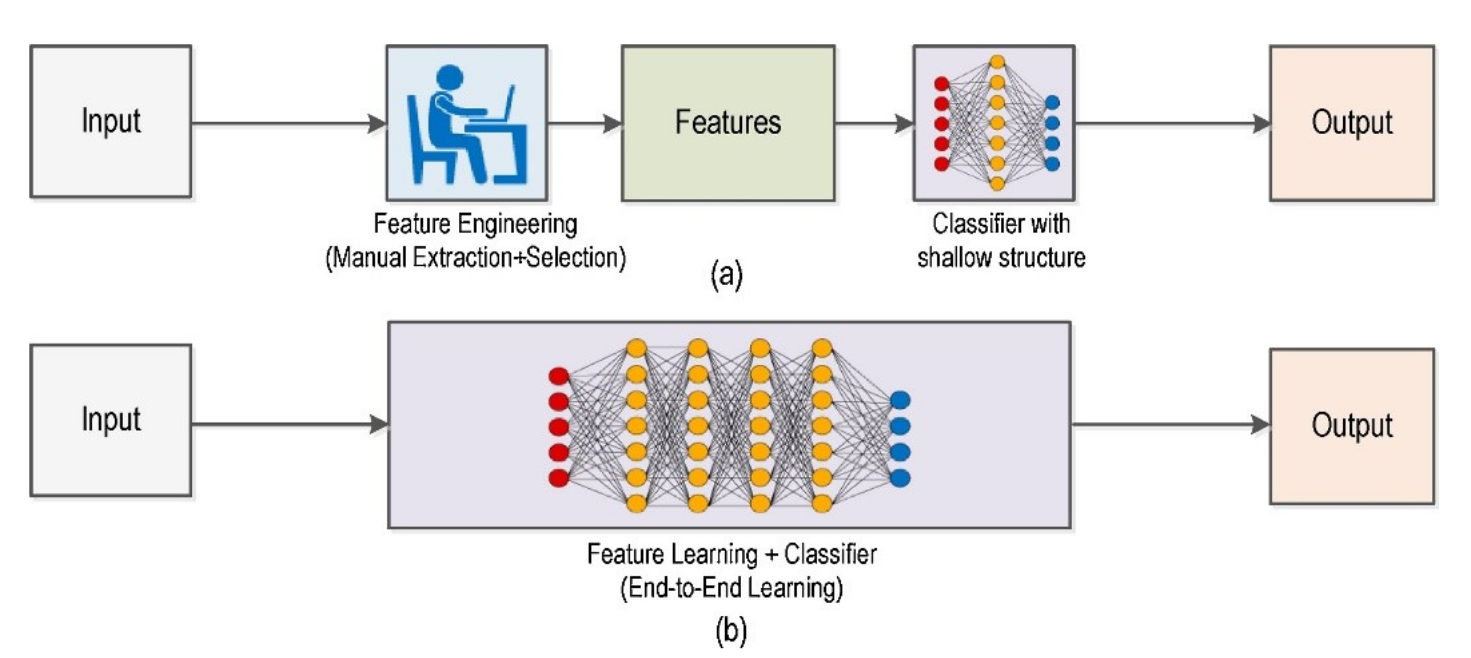
\includegraphics[width=115mm]{figures/dl_v_traditional.png}
\caption{Porównanie procesu budowania modelu rozpoznawania obrazów w~sposób deskryptywny (a) oraz za pomocą uczenia głębokiego (b) \cite{walsh19}.}
\label{fig:walsh19}
\end{figure}

Rozwój teorii sztucznych sieci neuronowych oraz technologii umożliwiających intensywne gromadzenie i~przetwarzanie danych zapoczątkowały nowe podejście w~sposobie rozwiązywania klasycznych problemów rozpoznawania obrazów. W~drugiej dekadzie XXI wieku konwolucyjne sieci neuronowe zdominowały konkursy klasyfikacji zdjęć \cite{imagenet} i~umożliwiły rozwiązywanie praktycznych problemów niegdyś uznawanych za nieosiągalne dla automatycznego przetwarzania. Ten imponujący postęp nie oznacza jednak końca dla tradycyjnych metod rozpoznawania obrazów.

Starsze, deskryptywne podejście w~analizie informacji polega na tworzeniu jawnego modelu matematycznego, który, zaczynając od surowych danych wejściowych, stopniowo odnajduje wcześniej ustalone wzorce coraz wyższego poziomu. W~przypadku klasyfikacji obrazów może to oznaczać przekształcenia na poziome sąsiedztwa pikseli i~przestrzeni barw, umożliwiające wykrycie „interesujących” cech. Na ich podstawie następnie tworzone są definicje klas obiektów służące do podejmowania decyzji będących ostatecznym rozwiązaniem problemu. Warto zauważyć, że tradycyjne metody przetwarzania obrazów działają z~taką samą skutecznością dla dowolnych danych wejściowych i~nie wymagają żadnej wiedzy związanej z~wysokopoziomowym zadaniem.

Natomiast analiza predykcyjna, reprezentowana przez uczenie głębokie, zastępuje stopniowy podział problemu całościowym podejściem bezpośrednio wiążącym dane wejściowe z~końcowym rezultatem. Pomimo, że również tutaj można dostrzec konstrukcję modelu „od szczegółu do ogółu”, to w~tym przypadku cechuje się ona wysokim stopniem samoorganizacji, pozwalającym na odkrycie reguł trudnych do jawnego zdefiniowania (i często także zinterpretowania) przez człowieka. Ceną tej elastyczności jest konieczność zapewnienia licznego zbioru przypadków o~znanych rozwiązaniach oraz ograniczenie skuteczności podejścia predykcyjnego do instancji podobnych do tych już zaobserwowanych.

Na podstawie powyższego porównania możemy zauważyć, że tradycyjne podejście do rozpoznawania obrazów nadal może liczyć na szerokie zastosowanie. Okazuje się ono zwyczajnie skuteczniejsze w~zastosowaniach wymagających działania na danych o~dużym zróżnicowaniu i~trudnych do opisania w~kategoriach klasyfikacji. Pozostaje również koniecznością, gdy brakuje odpowiedniej ilości danych treningowych \cite{walsh19}.

\subsubsection{Śledzenie obiektów (\emph{tracking})}
Zadanie śledzenia obiektów jest jednym z~najczęściej występujących elementów analizy nagrań: znając współrzędne określonego punktu w~momencie t, celem jest określenie jego położenia w~chwili t+1 \cite{medianflow}. Praktyka rozwiązywania tego problemu wskazuje jednak, że w~istocie wymaga on uwzględnienia dwóch zasadniczych procesów:
\begin{itemize}
    \item ruchu obiektu, modelowanego jako translacja jego współrzędnych,
    \item zmian wyglądu obiektu, uwzględniających również zmiany oświetlenia, zasłonięcie przez inne elementy, a~nawet przemieszczenie poza krawędź nagrania \cite{shi94}.
\end{itemize}

Zmiany pierwszego rodzaju, których udział dominuje przy analizie krótkich sekwencji, są skutecznie rozpoznawane przez minimalizację różnicy pomiędzy obszarem zainteresowania (region of interest) a~fragmentami następnej klatki. Różnica ta może być modelowana np. przez korelację \cite{mosse}, sumę kwadratów różnic (SSD - sum of squared differences) \cite{medianflow} czy projekcję wsteczną histogramu kolorów \cite{meanshift}.

Z kolei zmiany wyglądu obiektu nastręczają większych trudności, często powodując utratę pierwotnego obszaru zainteresowania. Fakt reprezentacji trójwymiarowej sceny przez dwuwymiarowy obraz w~oczywisty sposób pociąga za sobą utratę informacji pozwalającej na jednoznaczne rozpoznanie pożądanych punktów. W~celu uzupełnienia braku danych na temat pełnego stanu obiektów zaproponowano różnorodne podejścia:
\begin{itemize}
    \item Estymację rzeczywistej trajektorii na podstawie obserwacji zmian wcześniejszych pomiarów; klasycznym algorytmem tego rodzaju jest filtr Kalmana uwzględniający szum o~rozkładzie Gaussa \cite{kalman}.
    \item Monitorowanie różnicy pomiędzy pierwotnym obszarem a~aktualnie śledzonym, zdefiniowanej w~przestrzeni transformacji afinicznych (czyli zachowujących równoległość prostych) \cite{shi94}.
    \item Wykorzystanie faktu, że rzeczywista krzywa wyznaczona przez poruszający się obiekt jest odwracalna czasowo. Na przykład, gdy trajektoria obliczana jest przez znormalizowaną korelację krzyżową a~następnie porównywana z~analogicznym oszacowaniem dla zamienionej kolejności klatek \cite{medianflow}.
    \item Stopniowe budowanie modelu wyglądu obiektu z~wykorzystaniem technik uczenia
 maszynowego online. Można wyróżnić w~tym podejściu dwie ogólne metody: generatywną, która ocenia zgodność fragmentów obrazu z~ciągle aktualizowanym modelem docelowym, oraz dyskryminatywną, traktującą śledzenie jak problem klasyfikacji obszarów jako należących do obiektu bądź tła \citation{abbass20}.
\end{itemize}
\chapter{Technologie}

\section{System oznaczania zębów}
\subsection{Klient}

Vue.js, który został wykorzystany do realizacji modułu diagramu zębowego, to progresywny framework JavaScript umożliwiający implementację interfejsu użytkownika. Technologia ta powstała w~2014 roku i~cały czas się rozwija. Jej podstawowa biblioteka skupia się na tworzeniu warstwy widoku aplikacji i~w połączeniu z~bibliotekami pomocniczymi nadaje się do implementacji zaawansowanych aplikacji jednostronicowych. Aplikacje takie, właściwie nazywane Single-Page Application (SPA), charakteryzują się inną niż domyślna metodą ładowania stron. Rozwiązanie to pozwala na dynamiczną aktualizację jedynie poszczególnych komponentów aplikacji, unikając odświeżenia całej strony dla każdej, nawet małej zmiany.

\begin{figure}[ht!]
\centering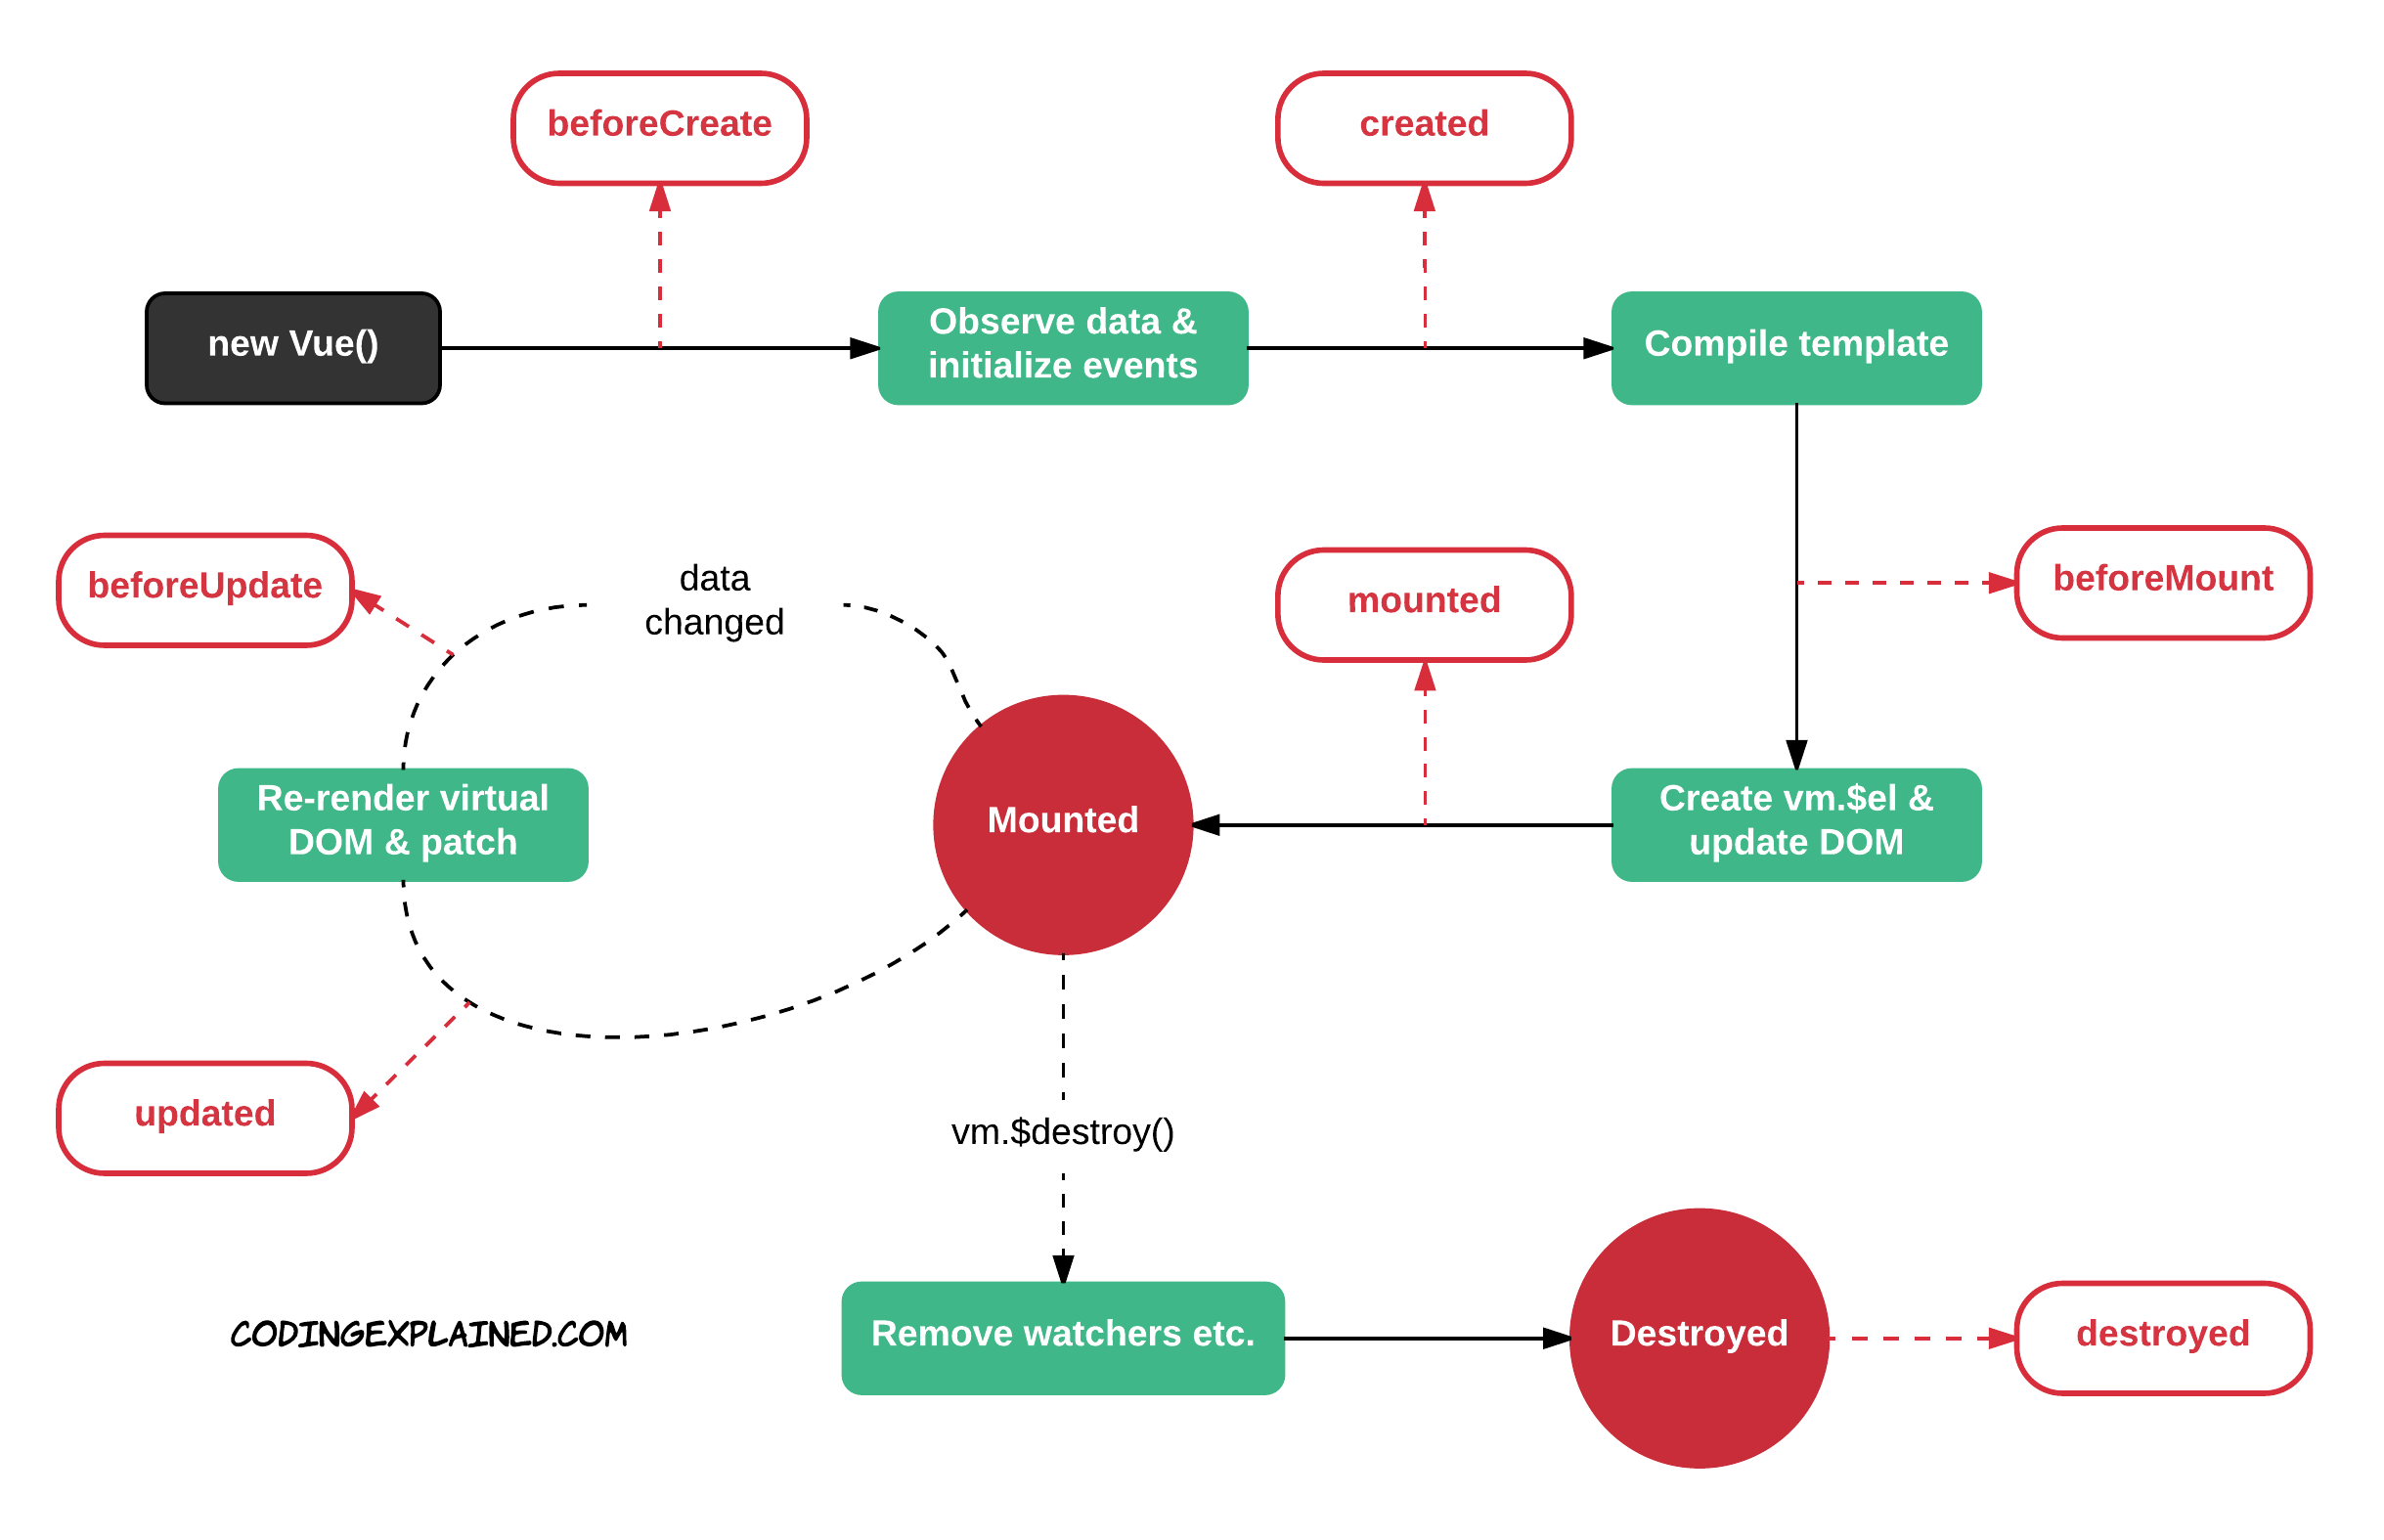
\includegraphics[width=\textwidth]{figures/Vue-instance-lifecycle-Page-1.png}
\caption{Diagram przedstawiający cykl życia instancji Vue\cite{vueLifeCycle}}
\label{fig:vuepopularity}
\end{figure}

Utworzenie aplikacji Vue jest jednoznaczne z~utworzeniem nowej instancji Vue (najczęściej oznaczanej jako vm), która składa się z~odrębnych komponentów. Działanie takiej aplikacji, a~właściwie poszczególnych jej komponentów, można w~prosty sposób przedstawić na diagramie, który nazywany jest cyklem życia Vue. Dla każdego komponentu aplikacji definiuje się zbiór właściwości oraz metod, które są wykorzystywane podczas działania programu. Pewien ściśle określony zbiór zmiennych jest reaktywny, co oznacza, że program wykrywa ich zmiany i~w razie ich edycji aktualizuje komponent używając nowo zdefiniowanych wartości i~ponownie go renderując.\cite{vuejs}

\begin{itemize}
\item koniecznie pros and cons - https://www.altexsoft.com/blog/engineering/pros-and-cons-of-vue-js/
\item w~kwestii diagramu działania Vue ,można opisać DOM - https://blog.logrocket.com/how-the-virtual-dom-works-in-vue-js/
\end{itemize}

\subsection{Serwer}
Serwer jest miejscem komunikacji wszystkich komponentów aplikacji. Jest odpowiedzialny za przetwarzanie żądań klienta oraz za łączność z~bazą danych i~z API do rozpoznawania mowy. Do implementacji serwera użyty został język Python oraz micro-framework Flask. 

\subsubsection{Flask}
Flask nazywany jest webowym mikro-frameworkiem. Przedrostek ,,mikro`` oznacza, że posiada prosty i~zajmujący mało miejsca pamięci rdzeń \cite{flaskdoc}. Jednakże jest zbudowany tak aby był modułowy i~bardzo elastyczny dla deweloperów. Flask nie posiada domyślnie takich funkcjonalności jak: ORM, arkusze walidacyjne, obsługa przekazywania plików czy systemów uwierzytelniania. Jak wspomniano wcześniej, framework posiada cechy, które pozwalają na proste użycie rozszerzeń. Dzięki czemu można uzupełnić funkcjonalności, w~sposób dopasowany do aktualnego projektu.
Flask jest frameworkiem WSGI. Oznacza to, że jest zgodny ze standardem języka Python o~nazwie PEP-3333. Standard zapewnia prostotę i~kompatybilność komunikacji między serwerem a~klientem dla aplikacji webowych w~języku Python\cite{pep3333}.

Budowa frameworka Flask bazuje na dwóch komponentach\cite{flaskdoc}:
\begin{itemize}
\item Jinja2 - silnik szablonów 
\item Werkzeug - biblioteka narzędzi do obsługi WSGI
\end{itemize}

Głównym zadaniem, do którego użyto powyższego frameworka jest obsługa żądań poprzez zaimplementowane węzły końcowe. Serwer jest uruchomiony w~tle i~działając nieprzerwanie, oczekuje na żądania. Serwer obsługuje zapytania POST w~komunikacji z~frontendem oraz bazą danych. Odpowiada również za rejestracje komend głosowych, połączenie z~API do rozpoznawania mowy oraz weryfikacji poprawności komend.

\subsubsection{MongoDB}
Technologią użytą do magazynowania oraz przetwarzania danych jest MongoDB. Jest to nierelacyjny system zarządzania bazami danych. Bazy MongoDB są przeznaczone do projektów gdzie istotna jest skalowalność oraz łatwy rozwój\cite{mongoDoc}. MongoDB jest zorientowane na dokumenty. Oznacza to, że zamiast tabel i~wierszy, jak w~relacyjnych bazach danych, używa kolekcji oraz dokumentów. Dokument jest tworzony w~stylu JSON, zawiera więc pary kluczy-wartości. Takie pary są podstawową jednostką danych w~technologi MongoDB. Kolekcje są zbiorem dokumentów.

Bazy danych MongoDB z~uwagi na typ NoSQL, posiadają pewne zalety:\cite{noSql}. 
\begin{itemize}
\item Duża skalowalność 
\item Elastyczny model obiektów danych
\item Przechowywanie masywnych danych
\item Prosta obsługa i~tanie utrzymanie
\item Szeroka konkurencja - duży wybór 
\item Duża liczba rozwiązań open-source
\end{itemize}
Bazy nierelacyjne nie są jednak najlepszym rozwiązanie do każdego projektu. Posiadają pewne wady w~stosunku do baz relacyjnych:\cite{noSql}. 
\begin{itemize}
\item Często z~uwagi na charakter open-source, nie posiadają pełnego wsparcia użytkownika
\item Nie posiadają wspólnego języka zapytań
\item Ewentualne błędy w~danych są trudne do wykrycia, z~uwagi na elastyczne modele danych
\end{itemize}

\begin{figure}[ht!]
\centering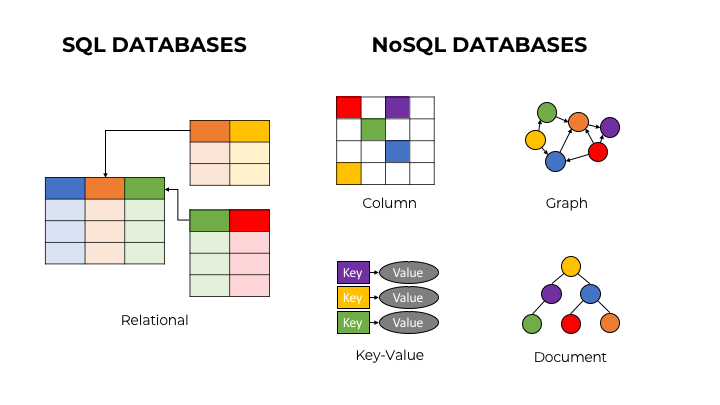
\includegraphics[width=\textwidth]{figures/sqlvsnosql.png}
\caption{Różnice między strukturami danych w~bazach danych typu relacyjnego (SQL) oraz bazach danych typu nierelacyjnego (NoSQL).}
\label{fig:sqlvsnosql}
\end{figure}

Wybór technologi MongoDB do realizacji projektu, był podyktowany prostotą wprowadzania zmian w~strukturze danych. W~szczególności możliwością rozszerzania aplikacji o~inne moduły, których model danych jest inny od obecnego w~aplikacji.
\subsection{Zewnętrzne API}
\subsubsection{Rozpoznawanie mowy}
Interfejs głosowy poprzez, który użytkownik może wprowadzać dane komendami głosowymi w~języku polskim, wymaga zaawansowanego rozwiązania. W~tym celu użyta została biblioteka Speech-Recognition w~języku Python\cite{pythonSpeech}. Główną funkcjonalnością biblioteki jest przetworzenie mowy na tekst. Wykorzystuje do tego kilka gotowych API dostępnych w~internecie. Do projektu zostało wybrane Google Speech Recognition API, które wykorzystuje Web Speech API\cite{webSpeechApi}.

Biblioteka \textbf{Python Speech Recognition} pozwala w~prosty sposób użyć swojej funkcjonalności w~projekcie. Cały proces zmieniający mowę na tekst, zawiera następujące kroki:
\begin{itemize}
\item Pobranie danych dźwiękowych z~mikrofonu bądź pliku
\item Przetworzenie danych dźwiękowych
\item Przesłanie żądania z~przetworzonymi danymi do Google Speech Recognition API
\item Odebranie odpowiedzi w~formie łańcucha tekstu
\end{itemize}

Wymogiem łączności z~API do rozpoznawania mowy jest łączność z~internetem. API jest dostępne publicznie do celów niekomercyjnych i~testowych\cite{webSpeechApi}. W~przypadku wydania aplikacji projektowej lub skomercjalizowania jej, jest możliwość zmiany API na Google Cloud API. Wiąże się to z~opłatami, jeżeli API przetwarza więcej niż 60 minut miesięcznie\cite{cloudSpeechAPI}. Każde żądanie jest rozumiane jako minimum 15 sekund. Można przyjąć, że w~aplikacji jedna komenda głosowa to jedno żądanie do API. Miesięcznie darmowe jest więc 240 komend głosowych. Za każde dodatkowe żądanie do 15 sekund należy zapłacić 0.006 dolara amerykańskiego. Przy kursie walutowym na poziomie 3,69 PLN za 1 USD, jedna komenda kosztuje 0,022 PLN.

W przypadku stomatologa, który realizuje 10 wizyt dziennie i~przy każdej z~nich wypowiada 6 komend głosowych oraz pracuje 22 dni robocze w~miesiącu. Lekarz wypowie 1320 komend miesięcznie, od czego należy odjąć 240 komend darmowych - co równa się 1080 żądań za kwotę 23,76 PLN. Dla tych samych założeń ale 10 komend poprawnych i~2 komend błędnych na wizytę, kwota miesięczna to 52,88 PLN.

\begin{figure}[ht!]
\centering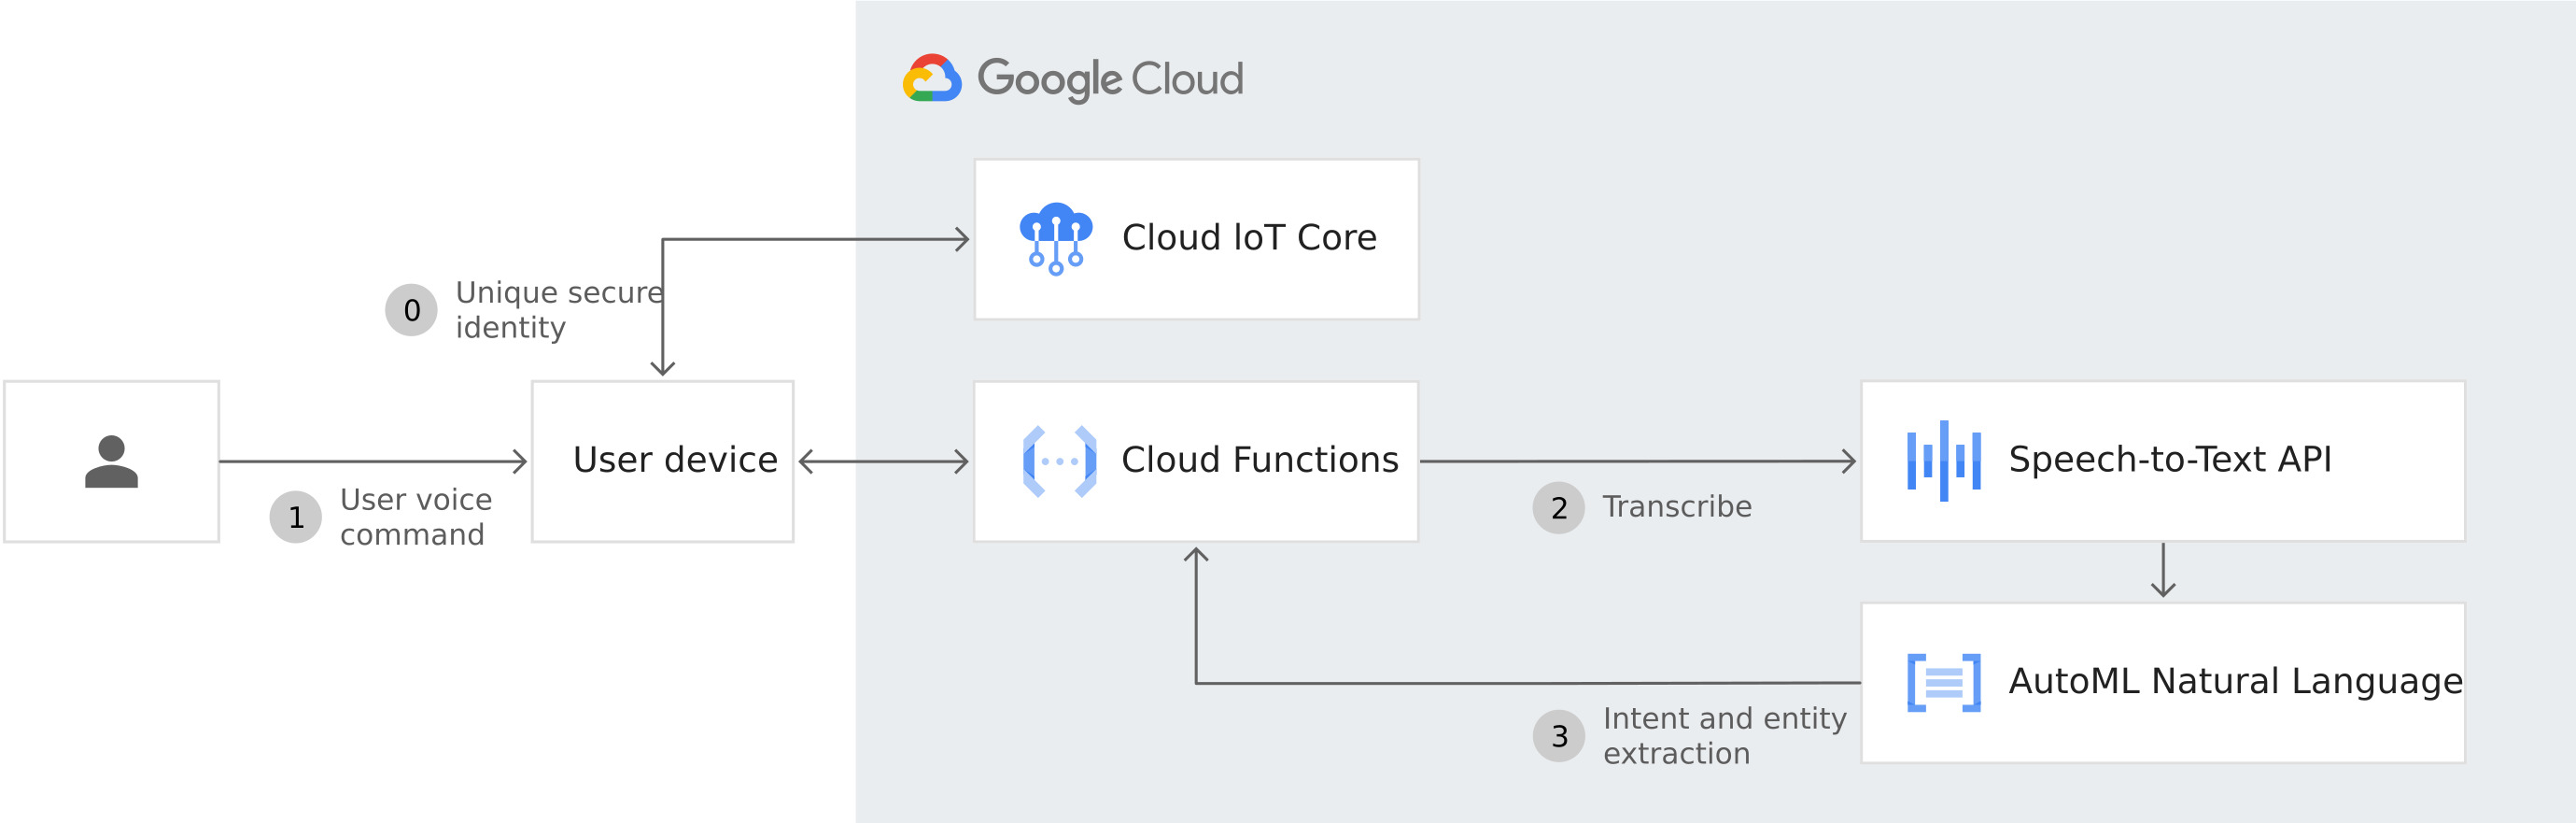
\includegraphics[width=\textwidth]{figures/googleCloudDiagram.jpg}
\caption{Diagram sposobu działania Google Cloud Speech Recognition API.\cite{cloudSpeechAPI}}
\label{fig:googleCloudDiagram}
\end{figure}



\section{Analiza odchylenia toru odwodzenia żuchwy}

\subsection{Wykorzystane biblioteki}

\subsubsection{Biblioteka NumPy}
NumPy (Numerical Python) to biblioteka open-source dostarczająca narzędzi do prowadzenia obliczeń na macierzach i tablicach wielowymiarowych \cite{numpy}. Z powodu wysokiej wydajności i prostoty przetwarzania na oferowanych przez siebie strukturach danych, NumPy stanowi dziś standard w niemal każdym naukowym i technicznym zastosowaniu języka Python. Tablice NumPy to w matematycznym sensie tensory, dlatego biblioteka umożliwia łatwą implementację modeli teoretycznych wyrażonych za pomocą algebry liniowej. Z uwagi na naturalną reprezentację, struktury danych oferowane przez bibliotekę w praktyce stanowią najpopularniejszy format transferu danych w naukowo-technicznym ekosystemie języka Python, czego dowodem może być łańcuch zależności przedstawiony na diagramie \ref{fig:numpy_applications}.

\begin{figure}
\centering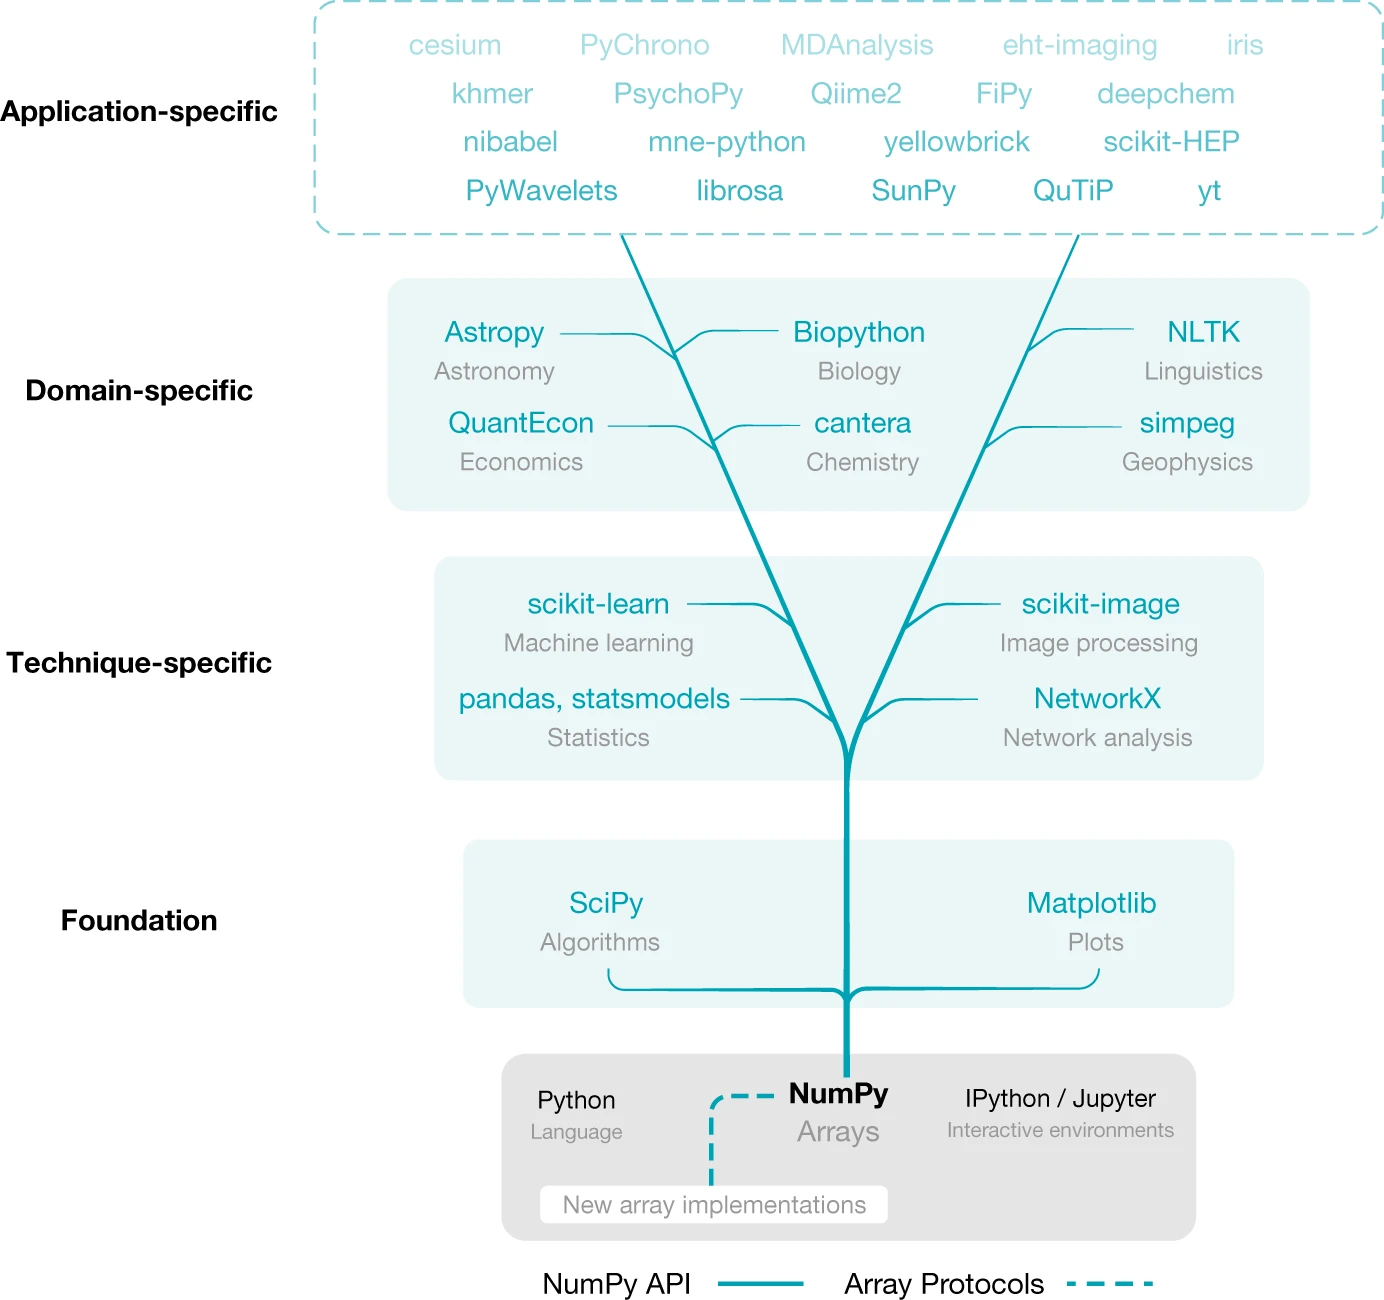
\includegraphics[width=100mm]{figures/numpy.png}
\caption{Miejsce biblioteki NumPy wśród narzędzi języka Python \cite{numpy}}
\label{fig:numpy_applications}
\end{figure}


\subsubsection{Biblioteka OpenCV}
Open Source Computer Vision Library\cite{opencv} to biblioteka funkcji zajmująca się przetwarzaniem obrazu oraz uczeniem maszynowym. Została zaprojektowana, aby dostarczyć łatwo dostępną infrastrukturę do tworzenia przetwarzających obraz aplikacji w~czasie rzeczywistym. Miała również przyspieszyć użycie podejścia maszynowego w~komercyjnych produktach. Dzięki oparciu na otwartym kodzie, pozwala firmą eksploatować i~rozwijać kod. Biblioteka OpenCV zawiera około 2500 zoptymalizowanych algorytmów, które oprócz klasycznych podejść do przetwarzania obrazów i~uczenia maszynowego, wyczerpują temat również w~zakresie najnowocześniejszych pomysłów. Algorytmy mogą zostać wykorzystane do np.:
\begin{itemize}
    \item Wykrycia i~rozpoznania ludzkiej twarzy
    \item Identyfikowania obiektów
    \item Przyporządkowywania ludzkich zachowań w~filmach
    \item Śledzenia poruszających się elementów w~filmach
    \item Uzyskania modelów 3D z~obiektów
    \item Składania obrazów w~jeden, aby pokazać obraz całej przestrzeni w~wysokiej rozdzielczości
    \item Znajdowania podobnego obrazu w~bazie danych
    \item Śledzenie ruchu gałek ocznych
    \item Usuwanie czerwonych gałek ocznych ze zdjęć
\end{itemize}
Biblioteka znajduje szerokie zastosowanie w~firmach i~grupach badawczych.
W projekcie zostały użyte różne funkcje z~biblioteki dotyczące śledzenia obiektów, wyświetlania i~obsługi filmów, transformację obrazu z~różnych przestrzeni barw.

\subsubsection{Biblioteka scikit-image}
scikit-image (skimage) to kolejna poświęcona przetwarzaniu obrazów biblioteka języka Python. Dostarcza ona algorytmów oraz narzędzi poświęconych badaniom, edukacji i zastosowaniom komercyjnym. Jej twórcy podkreślają prostotę interfejsu programistycznego i jakość dokumentacji, znacznie ułatwiające naukę zarówno w formie samodzielnej eksploracji, jak i zorganizowanych kursów. Biblioteka scikit-image rozpowszechniana jest w ramach bardzo liberalnej licencji \emph{Modified BSD}, zapewniającej pełną możliwość modyfikacji kodu, ale również wykorzystywania w zamkniętym oprogramowaniu. W obliczu faktu znacznego pokrywania się funkcjonalności scikit-image z OpenCV, warto podkreślić różnice pomiędzy tymi bibliotekami. Logika OpenCV zaimplementowana jest w językach C i C++, co powoduje bardziej proceduralny, niskopoziomowy sposób obsługi jej interfejsu dla języka Python. Z kolei scikit-image jest w pełni dopasowana do filozofii i stylu technologii Python, umożliwiając programowanie zgodne z podejściem imperatywnym lub funkcyjnym. Ponadto dostarcza ona nie tylko algorytmów z dziedziny widzenia komputerowego, lecz także przetwarzania obrazów medycznych i mikroskopowych \cite{skimage}.

\subsubsection{Biblioteka Tkinter}
Biblioteka Tkinter\cite{tkinter} to standardowe narzędzie w~języku Python, używane do tworzenia graficznego interfejsu użytkownika. Jest dostępny na większości platform Unix, a~także na systemach Windows.
Został wykorzystany, aby stomatolog mógł łatwo wybrać i~przetworzyć przechowywane na komputerze filmy.

\subsection{Interfejs programistyczny przetwarzania obrazów}

Zdjęcia i nagrania uzyskane metodami fotografii cyfrowej tworzone są w procesie naświetlania matrycy, tworzącej dyskretną reprezentację wizualną sceny. Z tego powodu wszystkie niskopoziomowe techniki przetwarzania obrazu zakładają implementację grafiki w formie rastrowej. Oznacza to, że dane przechowywane są w formie tablicy wielowymiarowej, w której najmniejszą jednostką jest piksel. Informacja o względnym położeniu punktów obrazu odwzorowana jest w indeksy poszczególnych pikseli, natomiast intensywność punktów kodowana jest w formie skalara (w przypadku obrazów monochromatycznych) lub wektora o trzech składowych (w reprezentacjach wielokolorowych).  

Współczesne kamery są w stanie zbierać ilości informacji znacznie przekraczające czułość ludzkiej percepcji. Co więcej obrazy przedstawiające rzeczywiste obiekty cechują się znaczną regularnością, w stosunku do wszystkich możliwych macierzy o danym kształcie \cite{image_svd}. Z tych względów wynaleziono bardzo wiele metod kompresji obrazów, i co za tym idzie, formatów plików do ich przechowywania. Standardowe narzędzia programistyczne (jak scikit-image czy OpenCV) zapewniają abstrakcję reprezentacji wczytywanego pliku i zwracają zdekompresowaną informację w formie tablicy liczb zmiennoprzecinkowych w ustalonej przestrzeni barw \cite{learning_opencv}.

Z racji tego, że filmy to zwyczajnie sekwencje obrazów o ustalonych odstępach czasowych, interfejs analizy nagrań definiowany jest zarówno w scikit-image, jak i w OpenCV, w formie strumienia klatek. Strumieniowy sposób przetwarzania pozwala pominąć kwestie długości nagrania czy liczby klatek na sekundę i przetwarzać kolejne próbki w identyczny sposób jak samodzielne obrazy. Oczywiście pożądane może być przechowywanie informacji o zmianach danych w czasie, ale realizuje się je poza interfejsem wczytywania nagrania.

\begin{figure}
    \centering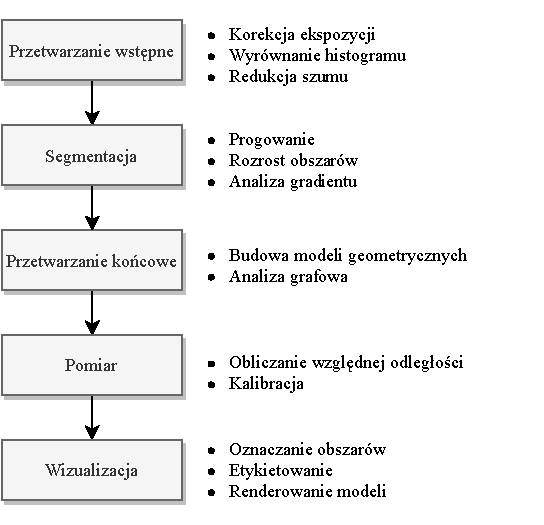
\includegraphics[width=100mm]{figures/Diagram przetwarzania.pdf}
    \caption{Diagram etapów przykładowego procesu przetwarzania obrazów}
    \label{fig:image_pipeline}
\end{figure}

Struktury danych będące wynikiem algorytmów wyższego poziomu niż wejściowe obrazy w większym stopniu zależą od decyzji twórców danej biblioteki. Często wykorzystywane są typowe kształty geometryczne, jednak ich implementacje w różnych bibliotekach mogą nie być ze sobą kompatybilne. Konieczne jest wówczas zachowanie ostrożności przy równoczesnym wykorzystaniu funkcji o różnych reprezentacjach obiektów mających tę samą interpretację (jak na przykład w przypadku prostokąta w bibliotekach scikit-image oraz OpenCV).



\chapter{Architektura}


\section{System oznaczania zębów}
W tym rozdziale opisano budowę aplikacji. Ważną częścią jest opis sposobu komunikacji między komponentami aplikacji oraz zestawienie modeli danych. Aplikacja jest złożona z~kilku komponentów:
\begin{itemize}
\item Klient
\item Serwer
\item Baza danych
\end{itemize}
Do każdego komponentu użyto innej technologii. W~celu zaimplementowania klienta użyto języka JavaScript oraz frameworka Vue. Do zbudowania serwera skorzystano z~języka Python i~mikroframeworka Flask. Baza danych jest na podstawie technologii MongoDB, czyli systemu bazodanowego typu NoSQL lub inaczej, nierelacyjnego.

Architektura aplikacji tego modułu w~ogólności jest architekturą typu klient-serwer.\cite{clientServer} Typ charakteryzuje się tym, że wielu użytkowników za pomocą klienta może korzystać z~serwisów udostępnianych przez serwer. Klient jest rodzajem aplikacji lub procesu, który wysyła oraz odbiera wiadomości od serwera. Przykładem klienta jest aplikacja uruchamiana w~przeglądarce pod danym adresem internetowym. Taki rodzaj klienta użyty jest w~module systemu oznaczania zębów.

\begin{figure}[ht!]
\centering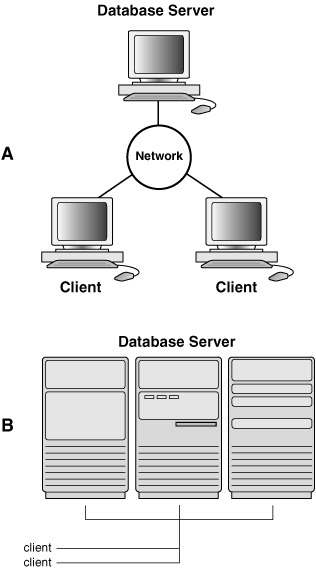
\includegraphics[width=75mm,scale=1.5]{figures/clientServerStanfor.jpg}
\caption{Przykładowy diagram budowy aplikacji, z~serwerem bazodanowym, o~architekturze klient-serwer.\cite{clientServerStanford}}
\label{fig:clientServerStanford}
\end{figure}

Dokładny sposób działania architektury klient-serwer jest następujący. Serwer jest serwisem uruchomionym w~trybie ciągłym. Serwer oczekuje na przyjęcie żądania od klienta. Po otrzymaniu żądania opracowuje odpowiedź i~zwraca ją klientowi. W~ogólności serwer zapewnia wykonanie wszystkich specyficznych i~złożonych operacji, aby aplikacja klienta nie była zależna od skomplikowanych wymagań sprzętowych i~oprogramowania. Serwer wystawiony w~sieci internetowej, fizycznie znajduje się w~zaawansowanej maszynie o~dużej mocy obliczeniowej. Natomiast użytkownik korzystający z~klienta, często operuje prostym komputerem osobistym bądź nawet urządzeniem mobilnym typu smartphone. Ważnym aspektem, który zachęca do używania architektury klient-serwer jest scentralizowanie dostępu do innych systemów poprzez serwer. Oznacza to, że klient nie musi mieć dostępu bezpośredniego do, przykładowo, baz danych. Cała komunikacja z~bazą danych jest poprowadzona przez serwer, który zapewnia prędkość i~bezpieczeństwo dostępu. Od aplikacji klienckiej wymagane będzie tylko uwierzytelnienie prawa dostępu do danej usługi prezentowanej przez serwer. Kolejnym istotnym aspektem jest dostęp do serwer przez wiele klientów na raz. Klienty mają możliwość w~sposób symultaniczny korzystać z~serwisów dostarczanych przez serwer. Aspekt ten wymaga od serwera dodatkowych systemów obsługi wielu zapytań od wielu klientów. Dzięki czemu klient może być prostszą i~zajmującą mniej miejsca pamięci aplikacją.


\subsection{Budowa aplikacji}
Architektura modułu, system oznaczania zębów, różni się od klasycznej architektury klient-serwer. Różnicą jest, że w~obecnej wersji oprogramowania pełna funkcjonalność działa tylko na lokalnej maszynie. Oznacza to, że serwer musi być uruchomiony na tej samej maszynie co klient. Jest to związane z~przetwarzaniem komend głosowych oraz urządzeń zewnętrznych potrzebnych do tego procesu. Nie zmieniają się inne zalety architektury klient-serwer. Nadal istnieje możliwość, w~obrębie maszyny z~serwerem, uruchomić kilka klientów i~działać na nich symultanicznie. Baza danych, nie musi być uruchomiona na tej samej maszynie. Aczkolwiek domyślne ustawienia łączności oczekują, że adres bazy będzie lokalny.

Komunikacja między komponentami odbywa się przy użyciu protokołu HTTP. Jest on często wykorzystywany podczas budowy aplikacji typu REST API. Moduł systemu oznaczania zębów jest zbudowany w~oparciu o~REST ale w~obecnej wersji nie spełnia wszystkich jego zasad. Styl REST odwołuje się do programistycznego interfejsu aplikacji, który spełnia opisane zasady architektury oraz pozawala na interakcję z~webowymi serwisami typu RESTful.\cite{restapibook} Akronim API oznacza zbiór definicji i~protokołów do budowania i~integracji aplikacji. Natomiast REST to zbiór ograniczeń i~zasad architektonicznych, nie jest to konkretny protokół lub standard. Deweloperzy zajmujący budową API, mogą w~wiele sposobów zaimplementować REST.

Działanie aplikacji typu REST jest proste i~pozwala na łatwe monitorowanie komunikacji. Kiedy żądanie klienta jest zrealizowane przez RESTful API, jest ono przekazywane razem z~treścią do węzła końcowego.\cite{restapi} Węzły końcowe są standardowo zlokalizowane na serwerze. Informacje przekazywane w~żądaniu są dostarczane w~postaci jednego z~kilku podstawowych formatów. Przykładowo formatami takimi są:
\begin{itemize}
    \item JSON
    \item HTML
    \item XML
\end{itemize}
Obecnie najczęściej używanym formatem jest JSON. Jego dużą zaletą jest czytelność plików, która pozwala zrozumieć zawartość osobom bez wiedzy technicznej. Istotną częścią żądania są nagłówki oraz parametry, które określa się metadanymi. Zawierają informacje takie jak: dane do autoryzacji, dane ciasteczek, pamięć podręczną, URI, kod statusu połączenia oraz inne dane.

Określenie konkretnej aplikacji typem RESTful\cite{restapibook}, wymaga od niej spełnienia kryteriów:
\begin{itemize}
    \item Architektura klient serwer - pozwala na odseparowanie interfejsu użytkownika od przechowywania danych. Pozwala na zwiększenie możliwości przenoszenia i~uruchamiania klienta na różnych platformach. Poprawia również skalowalność, upraszczając komponenty serwera.
    \item Bezstanowość - bezstanowa komunikacja klient-serwer oznacza, że żadne dane o~kliencie nie są przechowywane przez serwer między żądaniami. Zapewnia, że każde żądanie jest oddzielne i~niezależne od innych.
    \item Pamięć podręczna - buforowanie dostarczonych przez żądania danych po stronie klienta. Składowanie takich danych ma na celu zwiększenie prędkości przetwarzania żądań poprzez powtórne użytkowanie wcześniej zdobytych danych. Ustawienia tego procesu powinny mieć na uwadze, że część otrzymywanych danych może się różnić, nawet w~dwóch żądaniach do tego samego węzła końcowego na serwerze.
    \item System warstwowy - organizowanie każdego typu serwera, np. odpowiedzialnego za bezpieczeństwo czy równoważenie obciążenia, w~warstwy połączone ze sobą. Takie podejście pozwala na dużą skalowalności aplikacji. Klient komunikujący się, z~tak zbudowanym serwerem, nie jest w~stanie określić z~jaką warstwą jest aktualnie połączony.
    \item Jednolity interfejs - zastosowanie dokładnie określonego API pozwala na separację implementacji klient i~serwera. Styl REST podaje bardziej techniczne uwagi na temat budowania takiego interfejsu:
    \begin{itemize}
        \item Na podstawie pojedynczego żądania, serwer jest w~stanie zidentyfikować użytkownika. Standardowo w~tym celu umieszcza się w~wiadomości adres URI.
        \item Klient może manipulować otrzymanymi zasobami za pośrednictwem reprezentacji. Ponieważ reprezentacja zawiera wystarczającą ilość informacji, aby to zrobić.
        \item Wiadomości zwracane do klienta zawierają wystarczającą ilość informacji, aby opisać, jak klient powinien je przetwarzać. Przykładem jest ustawianie pola metadanych o~typie zawartości w~nagłówku żądania HTTP. Dla formatu JSON, pole to jest powinno być ustawione na 	,,application/json''.
        \item Dostępny jest hipertekst lub hipermedia. Po uzyskaniu dostępu do zasobu klient powinien mieć możliwość korzystania z~hiperłączy, w~celu znalezienia wszystkich dostępnych działań, które może wykonać. 
    \end{itemize}
    \item Kod na żądanie - wysyłanie kodu wykonywalnego z~serwera do klienta na żądanie. Pozwala na rozszerzenie funkcjonalność klienta. Ten punkt jest opcjonalny przy budowie aplikacji typu REST.
\end{itemize}

Budowa aplikacji modułu systemu oznaczania zębów spełnia część z~podanych wyżej kryteriów. Jest oparta na architekturze klient-serwer. Występuje komunikacja bezstanowa. Aplikacja jest za mała aby w~pełni korzystać z~systemu warstwowego, ale oddzielnie działa baza danych i~API do rozpoznawania mowy. Spełnione jest też założenie jednolitego interfejsu. Nie jest zaimplementowana możliwość korzystania z~kodu na żądanie. Pamięć podręczna nie jest w~pełni kontrolowana przez napisane oprogramowanie. 


\begin{figure}[ht!]
\centering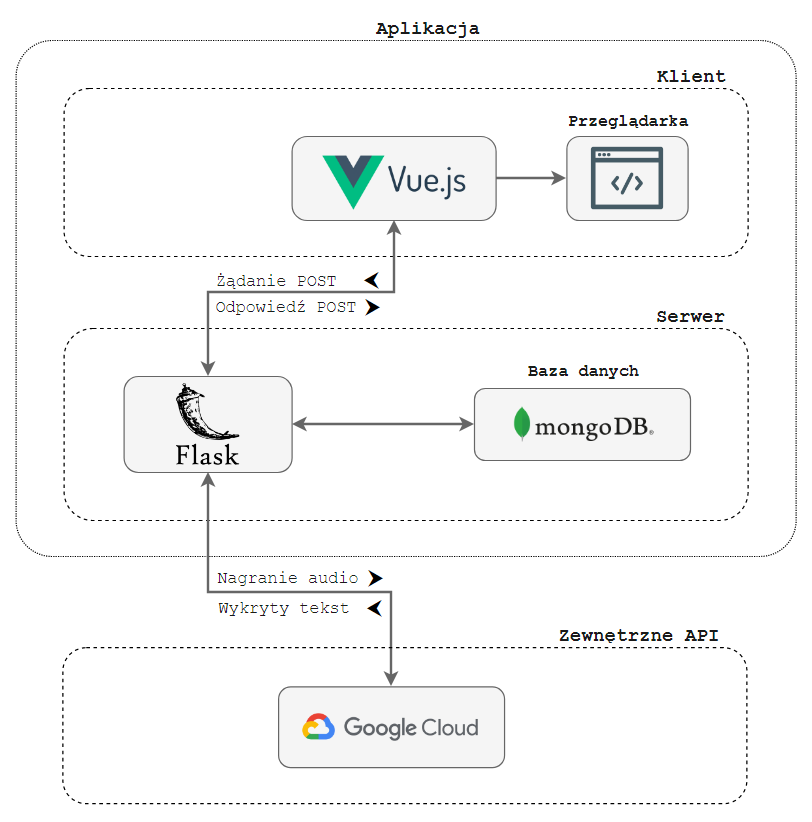
\includegraphics[width=140mm,scale=1.5]{figures/app.png}
\caption{Diagram budowy aplikacji modułu - system oznaczanie zębów.}
\label{fig:appArch}
\end{figure}

Na diagramie z~rysunku \ref{fig:appArch} jest przedstawiona budowa aplikacji oraz przepływy danych. Głównym komponentem jest serwer zrealizowany w~technologii Flask. Odpowiada on za obsługę żądań od klientów. Komunikacja odbywa się za pomocą żądań HTTP. Sposób budowy aplikacji jest oparty o~styl REST, którego szczegóły zostały opisane wcześniej.


Od strony serwera, za komunikację odpowiadają węzły końcowe. Każdy z~węzłów ma inny adres, w~celu  unikalności. Przykładowy węzeł końcowy, w~technologii Flask i~języku Python, podano poniżej:
\begin{lstlisting}
@app.route('/getPersonData', methods=['POST'])
\end{lstlisting}
Zakładając, że serwer uruchomiony jest na adresie 127.0.0.1, oraz że przyjmuje standardowy dla Flask port 5000. Pełnym adresem dla tego węzła jest:
\begin{lstlisting}
127.0.0.1:5000/getPersonData
\end{lstlisting}
W przykładzie widać również, że jest podane jakiego typu metoda HTTP obsługuje węzeł. W~tym module, w~prawie całej komunikacji, używana jest metoda POST. Nazwy węzłów zwyczajowo opisują operację wykonywaną przez serwis węzła. W~przykładzie taką operacją będzie pobranie danych osoby z~bazy danych i~dostarczenie ich, w~wiadomości zwrotnej, do klienta. 

Zgodnie z~diagramem z~rysunku \ref{fig:appArch}, komunikację w~aplikacji można podzielić na 3 kanały. Pierwszym kanałem jest połączenie serwera Flask z~klientem. Klient jest aplikacją uruchomioną na porcie 8080 w~przeglądarce internetowej. Jest to najważniejszy kanał komunikacji, ponieważ obsługuje żądania klienta. Na podstawie tych żądań wywoływanych jest większość operacji w~aplikacji. Serwer i~klient wymieniają między sobą wiadomości zawierające dane osób, które są pacjentami stomatologicznymi. Dokładny opis wiadomości znajduję się poniżej w~podrozdziale ,,Modele danych''. Drugim kanałem jest połączenie serwera Flask i~serwera bazy danych. Baza przechowuje dane pacjentów oraz parametry dotyczące chorób i~części zębów. Połączenie używane jest do dostarczania i~zapisywania danych na żądania klienta. Używane jest także przy komponowaniu komend z~tekstu otrzymanego z~interfejsu rozpoznawania mowy. Trzeci kanał jest między serwerem Flask a~zewnętrznym API. Połączenie to wymaga dostępu do internetu. Google Speech Recognition API przyjmuje na wejście plik audio nagrany poprzez mikrofon użytkownika. Plik zostaje przetworzony na tekst i~wysłany jako odpowiedź do serwera aplikacji. Jeżeli komenda zostanie uznana za poprawną, Flask przesyła ją do klienta. Frontend zrealizowany w~technologii Vue jest asynchroniczny, dzięki czemu zmiana wywołana komendą jest natychmiast widoczna w~przeglądarce internetowej. Zmiana nie jest w~tym momencie zapisana do bazy danych. W~celu zapisu nowych danych należy posłużyć się odpowiednim przyciskiem na widoku danych osobowych. 

\subsection{Modele danych}
W aplikacji modułu systemu oznaczania zębów dane przechowywane są nierelacyjnej bazie danych w~technologii MongoDB. Dane w~bazie zapisane są w~formacie JSON. JSON to format wymiany danych. \cite{json} Charakteryzuje się, tym że zawiera małą ilość pamięci danych, oraz że jest prosty do czytania i~tworzenia dla ludzi. Dodatkowo jest łatwy do przetwarzania i~generowania dla maszyn. Jako format tekstowy jest w~pełni niezależny od konkretnego języka programowania. Aczkolwiek jego konwencja bazuje na językach z~rodziny C, taki jak C, C++, Java czy Python. Wszystkie te właściwości sprawiają, że JSON jest dobrym językiem wymiany danych. 
\begin{figure}[ht!]
\centering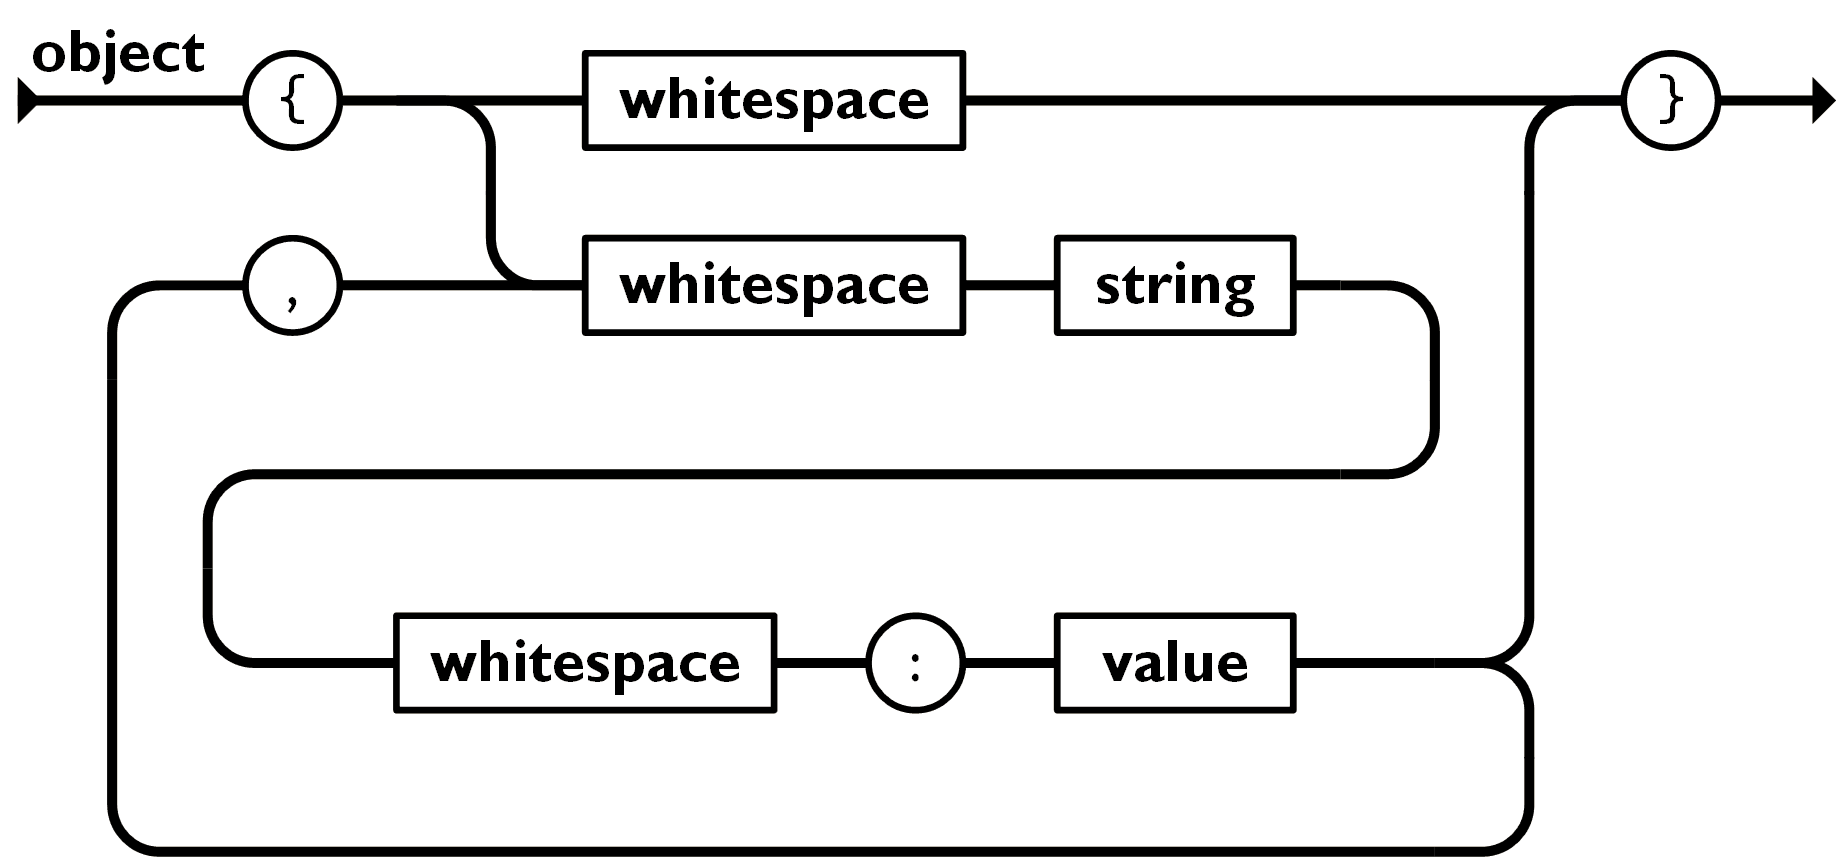
\includegraphics[width=145mm,scale=1.5]{figures/json1.png}
\caption{Diagram budowy podstawowego obiektu w~formacie JSON.}
\label{fig:jsonBuild}
\end{figure}
Diagram budowy obiektu w~formacie JSON jest zaprezentowany na rysunku \ref{fig:jsonBuild}. Dane zapisywane są przy pomocy klucza i~wartości oddzielonych dwukropkiem. Przykładem obiektu mogą być dane osobowe zawierające imię, nazwisko oraz PESEL. Taki obiekt prezentował by się w~formacie JSON jak poniżej.
\begin{lstlisting}
    {
        "imie" : "Jan",
        "nazwisko" : "Kowalski",
        "PESEL" : "87101912345"
    }
\end{lstlisting}
Format pozwala na prezentowanie bardziej skomplikowanych struktur, jak tablice obiektów:
\begin{lstlisting}
    "klienci" : [
        {
        "imie" : "Wojciech",
        "nazwisko" : "Sosnowski",
        "PESEL" : "87101912346"
        },
        {
        "imie" : "Krzysztof",
        "nazwisko" : "Tan",
        "PESEL" : "87101912347"
        }
    ]
\end{lstlisting}

Baza danych zawiera dwie kolekcje. Pierwszą jest ,,customers'', która zawiera wszystkie dane o~pacjentach. Dokument składa się z~czterech głównych obiektów:
    \begin{itemize}
        \item PersonalDetails - zawierający pola: imię, drugie imię, nazwisko, data urodzenia, PESEL, płeć
        \item ContactDetails - zwierający pola: numer telefonu, adres poczty elektronicznej oraz adres zamieszkania podzielony na nazwę ulicy, numer budynku, numer skrzynki pocztowej, kod pocztowy i~miasto 
        \item PermanentTeeth - zawiera dane 32 zębów stałych
        \item PrimaryTeeth - zawiera dane 20 zębów mlecznych
    \end{itemize}
Dodatkowo każdy dokument posiada pole daty wersji. Jest ono używane przy obsłudze wersji danych. Proces ten opisany jest w~dalszej części pracy. 
Ząb również jest obiektem. Technicznie, od strony programistycznej, ząb mleczny oraz ząb stały, są takim samymi obiektami. Ząb zawiera 5 pól. Każde z~pól oznacza jedną powierzchnię zęba. Nazwa powierzchni jest kluczem, a~wartością jest nazwa choroby. Dla powierzchni zdrowych, wartością jest wartość pusta, czyli ,,null''. Nazwy powierzchni są zakodowane jako wielkie litery, od A do E. Takie rozwiązanie jest podyktowane terminologią stomatologiczną, która dla tych samych powierzchni ma różne nazwy dla różnych zębów. Dla przykładu ząb o~numerze 11 ma powierzchnie sieczną, natomiast powierzchnia zęba o~numerze 15, na tej samej płaszczyźnie, to powierzchnia żująca. 
\begin{figure}[ht!]
\centering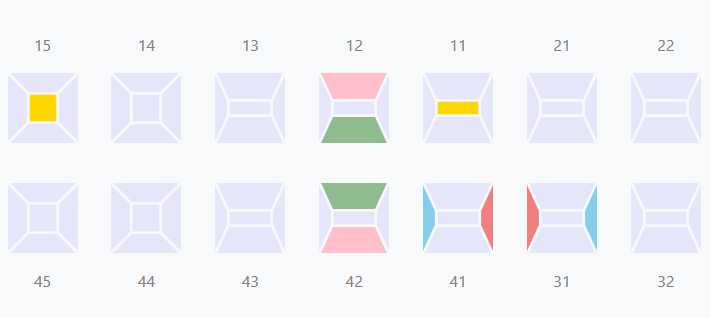
\includegraphics[width=145mm,scale=1.5]{figures/zeby.PNG}
\caption{Wycinek diagramu zębowego z~aplikacji.}
\label{fig:zeby}
\end{figure}
Na rysunku \ref{fig:zeby} kolorem żółtym oznaczono podany przykład. Innymi kolorami niż żółty, oznaczono powierzchnie, które mają takie same nazwy. Obrazuje to, że nazwa powierzchni zależy też od umiejscowienia zęba. Podobny problem jest z~terminologią chorób, które mają wiele nazw. Zaimplementowane rozwiązanie zostało dokładnie opisane w~rozdziale piątym, w~podpunkcie o~trudnościach oraz testowaniu.

Drugą kolekcją w~bazie danych, jest kolekcja ,,parameters''. Dokumenty zapisane w~niej, mają różne modele danych. Zawierają parametry i~słowniki. Pierwszy dokument zwiera słownik chorób. Oznacza to, że jeżeli choroba ma trzy nazwy, to jedna nazwa jest główna. Dwie pozostałe zostaną przetłumaczone na nazwę główną w~celu ujednolicenia nazw chorób na serwerze i~przy kolorowaniu diagramu zębowego. Tłumaczenie dotyczy tylko serwera. Dla użytkownika aplikacji oznacza to, że wypowiadając komendę głosową, może używać różnych nazw, tej samej choroby. Dla przykładu, ,,most'', ,,implant'' i~,,proteza'' oznaczane są takim samym kolorem na diagramie zębowym. W~celu uproszczenia komunikacji między serwerem a~klientem, wszystkie te nazwy tłumaczone są na słowo ,,proteza''. Poniżej zaprezentowano jak wygląda tłumaczenie w~formacie JSON dla podanego przykładu.
\begin{lstlisting}
    {
        "translation" : "most",
        "desease" : "proteza"
    }, 
    {
        "translation" : "implant",
        "desease" : "proteza"
    }, 
    {
        "translation" : "proteza",
        "desease" : "proteza"
    }
\end{lstlisting}
Drugi dokument zawiera analogiczny słownik dla nazw powierzchni zębów. Problem nazewnictwa powierzchni został opisany wcześniej oraz jest poruszony w~rozdziale piąty, w~temacie testowania aplikacji.
Kolekcja ,,parameters'' w~założeniu może być edytowana przez programy zewnętrzne, w~celu np. dodania translacji. W~związku z~tym, kolekcja ta jest aktualizowana przy każdy uruchomieniu serwera Flask.

Jak wspomniano wcześniej, w~dokumentach kolekcji ,,customers'' jest dodatkowe pole - data wersji. Jest to pole używane do procesu wersjonowania. Data, a~dokładniej czas, jest rejestrowany z~dokładnością do milisekund. Pozwala to na zapis kilku wersji tego samego dnia. Założeniem tego procesu w~aplikacji jest możliwość prześledzenia zmian na diagramie zębowym przez użytkownika aplikacji. Wersjonowanie dotyczy całych dokumentów. Każda nowa wersja jest nowym dokumentem. Nowa wersja powstaje po użyciu przycisku ,,Zapisz dane'' na widoku danych osobowych. Wersje można przeglądać na widoku diagramu zębowego. Data wersji jest jednym z~dwóch pól, które użyto do wyszukiwania dokumentów w~kolekcji ,,customers''. Drugim polem jest PESEL, który pozwala na zidentyfikowanie unikalnego pacjenta. Ze zbioru dokumentów z~tym samym numerem PESEL, jest wybierany na podstawie daty wersji np. najnowszy. W~związku, z~użytkowaniem pola PESEL do wyszukiwania, jest ono wymagane przy zapisie. Na polach PESEL, imię, nazwisko ustawione walidacje, które nie pozawalają utworzyć nowej wersji, bez ich wypełnienia. Reszta pól, czyli też wszystkie pola kontaktowe, jest opcjonalna i~nie blokuje zapisu.

\section{Analiza odchylenia toru odwodzenia żuchwy}
Polecam zrobić taki diagram jak u mnie, nawet jak będzie miałe dwa okienka, to zabiera dużo miejsca :)

W tej sekcji przedstawiono logiczną organizację modułów aplikacji mierzącej dewiację zgryzu. Następnie omówiono poszczególne etapy procesu analizy nagrań.

\subsection{Proces analizy nagrań}

Analizę, której poddawane jest nagranie można podzielić na trzy podzadania:
\begin{itemize}
    \item detekcję szczęk,
    \item śledzenie wykrytych szczęk w kolejnych klatkach,
    \item pomiar odchylenia na podstawie położenia szczęk.
\end{itemize}
Każdy kolejny etap korzysta z wyniku etapu poprzedniego, niezależnie od wewnętrznej logiki działania. Możliwe zatem było zaimplementowanie ich jako osobnych modułów o dość znacznej autonomii. W dalszej części rozdziału znajduje się opis działania każdego z nich.

\subsection{Etapy detekcji szczęk pacjenta}

Detekcja zębów na klatkach nagrania przebiega w sposób wielostopniowy: początkowe przekształcenia intensywności poszczególnych pikseli służą wyodrębnieniu regionów zainteresowania, z których wybierane są te najbardziej zgodne z kryteriami modelującymi pożądane cechy. Prostokątne obszary będące wyjściem modułu detekcji ostatecznie zyskują w logice aplikacji wyższego poziomu semantyczną interpretację  szczęk pacjenta. Poniżej omówiono szczegóły każdego etapu pracy detektora.

Nagrania wczytywane z pliku domyślnie reprezentowane są przez bibliotekę OpenCV w przestrzeni barw BGR \cite{opencv_colors}. Istotnym utrudnieniem w rozpoznawaniu obiektów na obrazach jest zmienność oświetlenia, która w reprezentacji BGR wpływa na wszystkie trzy składowe pikseli. Aby w łatwiejszy sposób operować na kolorach będących 'immanentną' cechą obiektów, obraz przekształcany jest w przestrzeń kolorów HSV, w której jasność (V -- \emph{value}) rozpatrywana jest niezależnie od odcienia (H -- \emph{hue}) i nasycenia koloru (S -- \emph{saturation}).  

Z wstępnego oglądu przekazanych nagrań wynika, że rozkład każdej z trzech składowych kolorystycznych obrazu nie zawiera podziału na wyraźne klasy. W istocie, wartości pikseli należących do zębów pacjenta pokrywają się z tymi odpowiadającymi skórze lub przyrządom dentystycznym. Z tych względów na etapie początkowej segmentacji wykorzystywany jest fakt, że w większości przypadków widoczne są dziąsła otaczające pożądany obszar zębów. Zatem progowanie eliminujące piksele o wyraźnie dominującym odcieniu czerwonym umożliwia podział obrazu na rozłączne obszary zębów oraz reszty twarzy \ref{fig:threshold}.

\begin{figure}
    \centering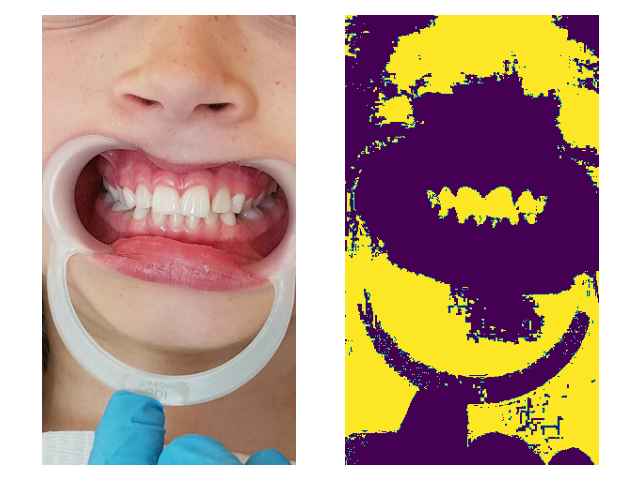
\includegraphics[width=75mm,scale=1.5]{figures/threshold.png}
    \caption{Progowanie obrazu według wartości odcienia}
    \label{fig:threshold}
\end{figure}

Po wykorzystaniu informacji zawartych w rozkładzie kolorów otrzymywana jest maska binarna zawierająca regiony potencjalnie będące szczękami, które na dalszym etapie poddawane są analizie z skupionej na kształcie i położeniu.  

Na etapie definiowania kryteriów, niestety, konieczne było poczynienie założeń w kwestii rotacji oraz skali obiektów na nagraniach, co ogranicza ogólną skuteczność detektora, jednak nie w przypadku nagrań dostarczonych na etapie rozwoju oprogramowania.  
Kroki procesu eliminacji potencjalnych regionów przedstawione są na rysunku \ref{fig:selection}. Najpierw (kolumna a), z maski usuwane są regiony o powierzchni przekraczającej maksymalną wartość,  przylegające do krawędzi obrazu (warunek rozmiaru jest konieczny, ponieważ może zdarzyć się, że fragment szczęki wykroczy poza zakres klatki). Następnie eliminowane są segmenty zbyt małe, aby uznać je za regiony odpowiednie do śledzenia (b). Pozostałe fragmenty oceniane są ze względu na wypukłość (\emph{solidity}), będącą stosunkiem pola obszaru do pola jego otoczki wypukłej \cite{regionprops}. Ponieważ zęby ukazane w sposób frontalny stanowią zwarty, wypukły kształt, wykluczone zostają regiony zbyt wklęsłe (c). W kolejnym kroku badana jest orientacja segmentów (d), czyli stosunek krótszej osi obrazu do osi wielkiej elipsy odpowiadającej badanemu segmentowi \cite{regionprops}; pozostawiane są tylko regiony o wystarczająco niskiej wartości tego kąta. Ostatnim etapem selekcji jest odrzucenie regionów oddalonych od środka nagrania.

\begin{figure}
    \centering 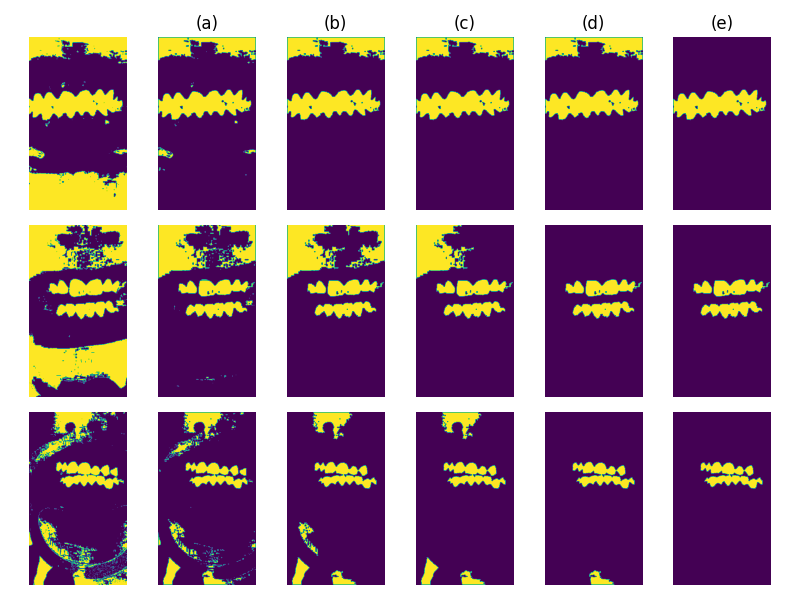
\includegraphics[width=140mm]{figures/selection.png}
    \caption{Rezultaty selekcji potencjalnych regionów na podstawie: (a) maksymalnego rozmiaru i przylegania do krawędzi, (b) minimalnego rozmiaru, (c) wypukłości, (d) orientacji, (e) odległości od środka}
    \label{fig:selection}
\end{figure}

Ostatnią kwestią objętą przez algorytm detekcji są sytuacje stykania się szczęk. Przetwarzanie omówione do tego momentu pozostawia zamknięte szczęki jako jeden region, co oczywiście uniemożliwia odpowiednie śledzenie ich ruchu. Z tego powodu przeprowadzana jest procedura wykrycia linii mogących stanowić krawędzie sieczne szczęk i podziału regionu wzdłuż owych linii. Wymienione poniżej etapy tego procesu zostały zilustrowane na rysunku \ref{fig:line_split}.

Na początku stosowany jest filtr Sobela, mierzący gradient intensywności pikseli wzdłuż twarzy (\ref{fig:line_split} a), co powoduje wyeksponowanie prostopadłych krawędzi (tj. punktów o odpowiednio wysokiej wartości gradientu). Z otrzymanego obrazu następnie otrzymywane są współrzędne linii wykrytych za pomocą transformacji Hougha (b). Znalezione odcinki muszą spełniać kryteria minimalnej długości i maksymalnej przerwy pomiędzy pikselami, dlatego możliwe jest, że na regionie nie zostaną wykryte odpowiednio wyraźne linie i przetwarzanie zakończy się. W przeciwnym wypadku spośród znalezionych odcinków wybierany jest ten, którego środek znajduje się najbliżej środka regionu, ale nie dalej niż 25\% odległości do krawędzi. Ostatecznie, obszar dzielony jest wzdłuż otrzymanej linii (c).

\begin{figure}
    \centering 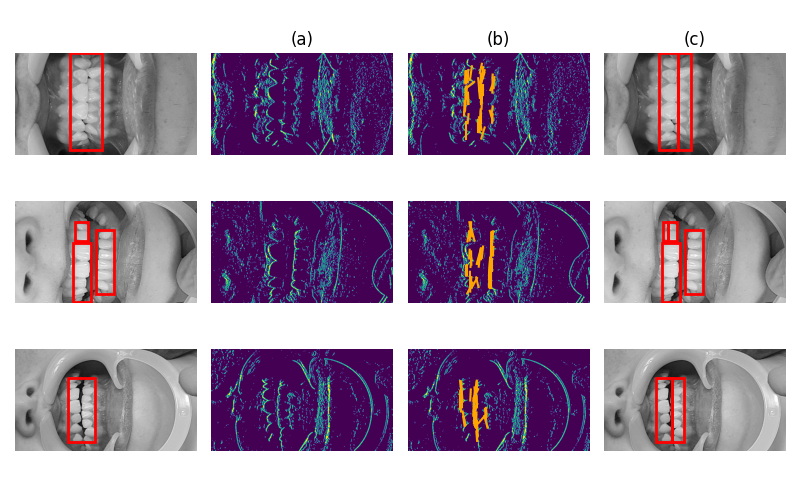
\includegraphics[width=140mm]{figures/line_split.png}
    \caption{Etapy podziału regionów: (a) wykrywanie krawędzi, (b) wykrywanie linii, (c) otrzymane nowe regiony}
    \label{fig:line_split}
\end{figure}

\subsection{Śledzenie szczęk}

Z formalnego punktu widzenia śledzenie oraz detekcja dostarczają odpowiedzi na to samo pytanie: Które piksele nagrania należą do obiektu będącego przedmiotem zainteresowania, a które nie? Faktycznie, w niektórych zastosowaniach dla każdej klatki wykorzystuje się jeden, ten sam algorytm detekcji, oznacza to jednak pominięcie informacji możliwej do uzyskania z poprzednich obserwacji. Poprawę wydajności, a nierzadko również skuteczności, przynosi zastosowanie algorytmu przewidującego trajektorię obiektu na podstawie informacji o jego położeniu w poprzednich klatkach, czyli trackera. W aplikacji zastosowano podejście, w którym śledzenie i detekcja wzajemnie się uzupełniają, czego szczegóły omówiono poniżej.  

Rdzeniem procesu śledzenia jest implementacja algorytmu MedianFlow dostarczona w bibliotece OpenCV \cite{opencv_trackingAPI}. Twórcy biblioteki zadbali o zapewnienie wspólnego interfejsu każdemu z oferowanych trackerów. Zatem to, który dokładnie algorytm wykorzystywany jest przez aplikację może zostać bardzo łatwo poddane modyfikacji, dzięki zastosowaniu wzorca projektowego strategii. Taka, oparta na technice wstrzykiwania zależności, architektura pozwoliła na sprawdzenie skuteczności wielu dostępnych algorytmów śledzenia bez konieczności zmiany pozostałego kodu.  

Poza samym aktualizowaniem trackera, przeprowadzana jest również walidacja zwracanych przez niego trajektorii szczęk. Powszechnym problemem takich algorytmów jest stopniowe "gubienie" śledzonego regionu, zwykle powodowane zmianą jego wyglądu lub widoczności. Z tego powodu, w regularnych odstępach czasu uruchamiana jest ponowna detekcja szczęk, której wynik następnie porównywany jest z regionami aktualnie wskazywanymi przez tracker. Miarą jakości wykorzystywaną w tej ocenie jest korelacja histogramów regionów odpowiadających szczękom. Jeśli wynik nowej detekcji cechuje się istotnie wyższą wartością tego kryterium oraz któryś z nowo znalezionych obszarów nie pokrywa się z żadnym z poprzednich w więcej niż 40\%, to aktualizowana jest para śledzonych regionów. Można taką sytuację interpretować jako utratę przez algorytm śledzenia trajektorii którejś ze szczęk.

\subsection{Pomiar dewiacji}

Po ustaleniu położenia szczęk, ostatnim etapem analizy jest obliczenie odchylenia dolnej szczęki względem pionowej trajektorii ruchu.
\chapter{Aplikacja}
Projekt zaczęto realizować w~lipcu 2020. Prace koncepcyjne oraz pozyskiwanie wiedzy zrealizowano w~sierpniu 2020, a~wynikiem tych działań było uruchomienie tablicy Trello. Trello to internetowy serwis, którego główną funkcją są tablice organizacji projektów. Tablica zawierała zadania deweloperskie, ale także organizacyjne. Cały projekt był prowadzony w~metodyce Scrum. Metodyka została dostosowana do charakteru oraz wielkości projektu. W~pierwszej połowie projektu regularne spotkania odbywały się co dwa tygodnie. W~drugiej połowie, gdzie przeważały szczegółowe zadania techniczne, spotkania odbywały się co tydzień. W~celu przechowywania kodu oraz kontroli wersji użyto technologii Git i~GitHub.
\section{System oznaczania zębów}
\subsection{Wymagania}
Podczas planowania projektu założono minimalne wymagania produktowe - MVP. Wymagania minimalne były kluczowym dokumentem przy regularnym planowaniu prac. Dla systemu oznaczania zębów postawiono takie założenia:
\begin{itemize}
    \item Diagram zębowy z~możliwością wprowadzania danych za pomocą myszki
    \item Przechowywanie informacji w~bazie danych
    \item Eksportowanie danych
\end{itemize} 
Stworzono diagram zębowy w~nowoczesnym stylu graficznym. Wprowadzanie danych jest możliwe za pomocą myszki ale także za pomocą interfejsu głosowego. Komendy głosowe pozwalają lekarzowi uzupełniać diagram zębowy podczas wizyty pacjenta. Taka funkcjonalność nie pojawia się w~innych tego typu produktach na rynku polskim. Dane są przechowywane w~nierelacyjnej bazie danych. Użyto technologii MongoDB. Zaletą nierelacyjnej bazy jest łatwość w~zmienianiu modeli i~struktur danych. Eksport danych jest możliwy na dwa sposoby. Pierwszy dotyczy udostępniania danych, zawartych na diagramie zębowym, pacjentowi. Sposób polega na możliwości wydrukowania diagramu do pliku PDF albo, wprost poprzez drukarkę sieciową, do formy papierowej. Podsumowując, spełniono minimalne wymagania produktowe. Jest to wskazanie na poprawne poprowadzenie projektu. 

Innymi wymaganiami, które opisano we wczesnym etapie projektu, były wymagania pozafunkcjonalne. Określono takie wymagania jak:
\begin{itemize}
    \item Użyteczność - możliwość przyswojenia działania systemu w~ciągu jednej godziny
    \item Kompatybilność - konieczność działania na każdej współczesnej przeglądarce internetowej
    \item Łatwość utrzymania - możliwość rozbudowania aplikacji o~dodatkowe moduły
    \item Bezpieczeństwo - uwierzytelnianie i~autoryzacja przed dostępem do danych
\end{itemize} 
W celu spełnienia założenia użyteczności zwrócono uwagę na prosty projekt graficzny. Cała aplikacja działa w~języku polskim, w~tym interfejs głosowy. Najbardziej skomplikowanym systemem dla użytkownika jest wprowadzanie komend głosowych. Sporządzono film instruktażowy oraz instrukcje użytkowania z~przykładami. Wymaganie kompatybilności zostało rozwiązane przez użycie nowoczesnych technologii opisanych w~rozdziale trzecim. Aplikacja została przetestowana, z~wynikiem pozytywnym, na sześciu nowoczesnych przeglądarkach. Opis testów jest zawarty w~dalszej części pracy. Łatwość utrzymania spełniono poprzez zbudowanie aplikacji na podstawie stylu REST. Aplikacja za pomocą interfejsu i~systemu węzłów końcowych, jest w~stanie rozszerzyć swoją funkcjonalność w~prosty sposób. Wymaganie bezpieczeństwa nie zostało spełnione. Ze względu na niedokładne oszacowanie poziomu skomplikowania implementacji systemów uwierzytelniania i~autoryzacji.

Wymaganie użyteczności, zostało opracowane w~dodatkowy, rozszerzony sposób na podstawie ISO25010. Poczyniono założenia:
\begin{itemize}
    \item Rozpoznawalność zastosowania - ściśle określona funkcja oprogramowania
    \item Łatwość nauczenia się - prostota aplikacji oraz użycie grafik branżowych, dobrze znanych potencjalnym klientom
    \item Ochrona użytkownika przed błędami - prostota aplikacji oraz zastosowanie walidacji pól
    \item Estetyka interfejsu użytkownika - zastosowanie najnowszych technologii, ale ważniejsza jest funkcjonalność
    \item Dostępność personalna - produkt ma sprecyzowaną grupę odbiorców, którzy posiadają podobne umiejętności
\end{itemize} 
Wszystkie z~opisanych powyżej założeń zostały spełnione. Dokładniejsza analiza funkcjonalności została opisana w~pracy wcześniej.


\subsection{Design}

Podczas tworzenia projektu graficznego modułu diagramu zębowego skupiono się na estetyce interfejsu użytkownika oraz jego nowoczesnym designie. Położono także nacisk na możliwie prostą formę ekranów, by ich obsługa nie była dla użytkownika barierą, ale by okazała się jak najbardziej intuicyjna. Szczególną uwagę skupiono na wyglądzie pojedynczego zęba oraz całego diagramu.

Moduł diagramu zębowego składa się z~dwóch głównych części. Pierwszą z~nich jest ekran prezentujący dane osobowe oraz kontaktowe pacjenta. Układ formularza jest przejrzysty i~dzięki takiemu rozwiązaniu - prezentacji danych w~edytowalnych polach - użytkownik jest w~stanie w~prosty sposób przeglądać i~jednocześnie aktualizować wcześniej wprowadzone dane w~jednym miejscu. Obowiązkowe do uzupełnienia dane w~formularzu są walidowane. Sprawdzana jest poprawność nanoszonych zmian, by dodatkowo ułatwić pracę użytkownikom i~pomóc im uniknąć błędów oraz związanych z~nimi ewentualnych konsekwencji.

Drugi ekran pozwala na prezentację oraz edycję danych dotyczących stanu uzębienia pacjenta. Projekt graficzny diagramu zębowego wykorzystanego w~aplikacji powstał na podstawie istniejących diagramów papierowych (Rysunek \ref{fig:karta}) oraz cyfrowych (Rysunek \ref{fig:diagramy}) używanych w~gabinetach stomatologicznych, a~także na podstawie konsultacji z~czynnym zawodowo stomatologiem. Ważne było, by był on jak najbardziej zbliżony do diagramów już wykorzystywanych w służbie zdrowia, tak by ułatwić pracę i~naukę obsługi nowego oprogramowania stomatologom, ale jednocześnie, by sprawdził się w~aplikacji desktopowej.

\begin{figure}[t!]
\centering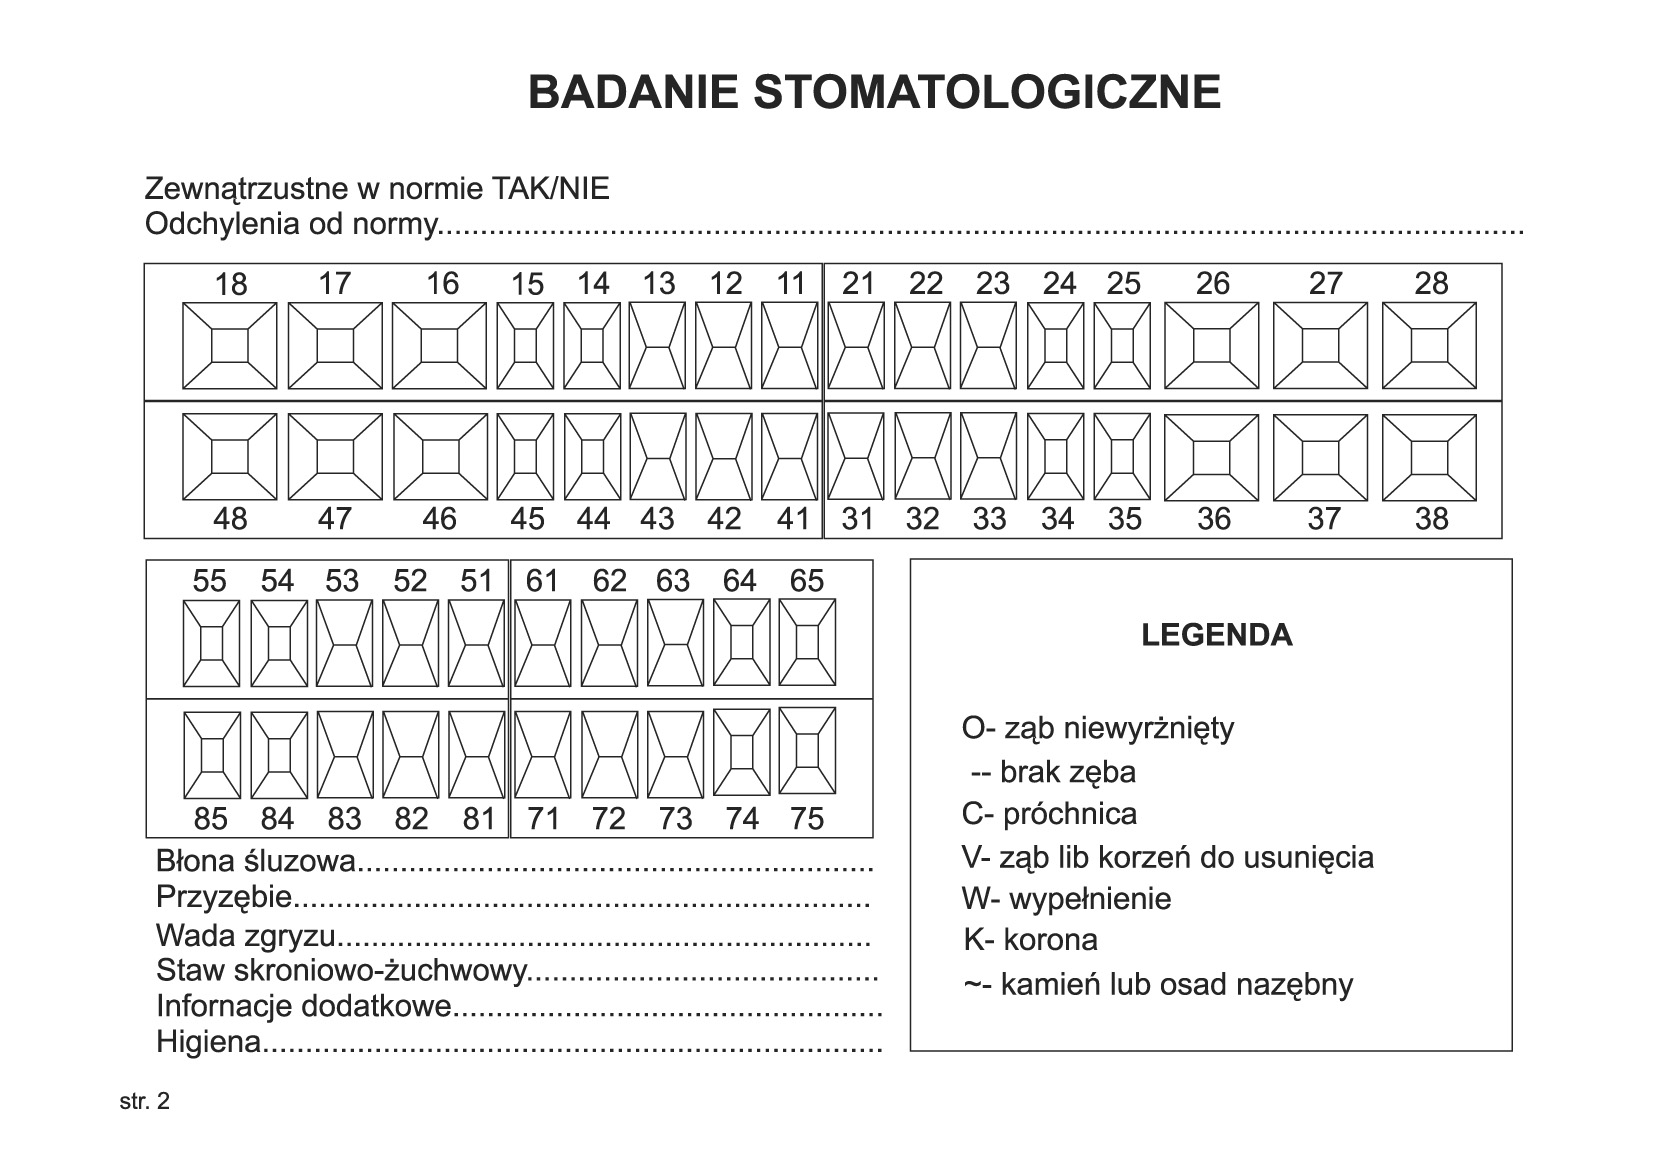
\includegraphics[width=\textwidth]{figures/karta.jpg}
\caption{Przykładowy diagram papierowy wykorzystywany w gabinetach stomatologicznych.\cite{Roydental}}
\label{fig:karta}
\end{figure}

\begin{figure}[t!]
\centering
\subfloat Diagram zębowy w programie eRUM\cite{eRUM}{\label{odnosnik}
\includegraphics[width=\textwidth]{figures/eRum.png}}
\quad
\subfloat Diagram zębowy w systemie Mediporta\cite{Mediporta}{\label{odnosnik}
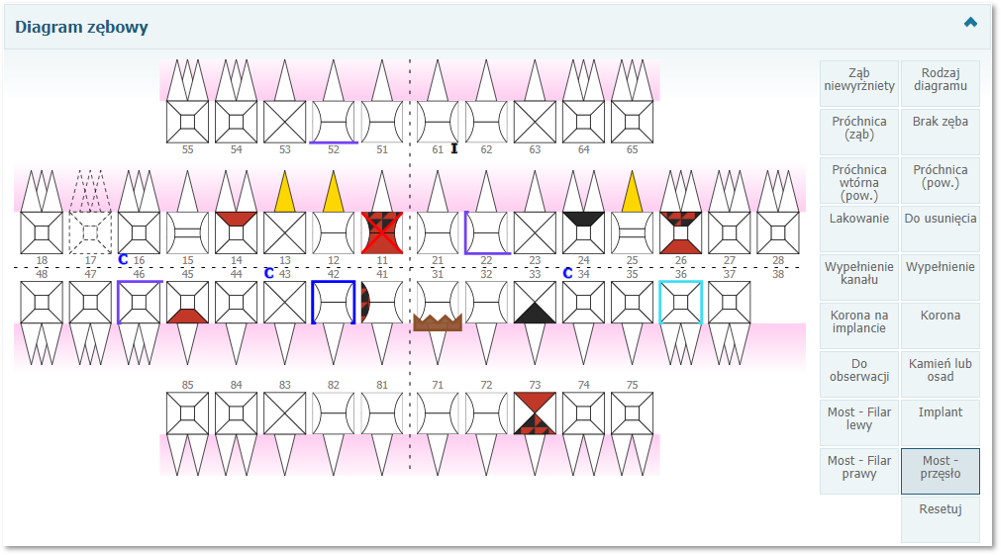
\includegraphics[width=\textwidth]{figures/mediporta.png}}
\caption{Diagramy wybranych aplikacji ułatwiających pracę stomatologom.}
\label{fig:diagramy}
\end{figure}

Diagramy wykorzystywane przez stomatologów bazują zarówno na kwadratowym jak i~okrągłym schemacie opisu zęba. Przy wyborze kształtu opisu wykorzystanego w~aplikacji kierowano się łatwością zaznaczania - możliwością szybkiego wyboru jednego elementu myszką, przejrzystością prezentowanych danych oraz ich estetyką. Ostatecznie w~aplikacji wykorzystano kwadratowy opis poszczególnych zębów. Każdy ząb składa się z~pięciu odrębnych części reprezentujących jego powierzchnie. By zwiększyć czytelność schematu, inaczej przedstawiono siekacze i~kły obu łuków - zwracając uwagę na ich nieduży brzeg sieczny, a~inaczej przedtrzonowce oraz trzonowce, uwydatniając ich powierzchnie zgryzowe.

Podczas tworzenia aplikacji i~projektowania jej interfejsu dużo uwagi poświęcono także detalom. Operacje wykonywane przez użytkownika są często potwierdzane i~opisywane w~widocznym miejscu przez system, by informować na bieżąco o~wprowadzanych zmianach. Takie elementy interfejsu pomagają w~prawidłowym użytkowaniu programu i~w pewien sposób prowadzą użytkownika. Co ważne, osoby korzystające z~aplikacji otrzymują także dodatkowe komunikaty podczas korzystania z~interfejsu głosowego dostępnego w~aplikacji.

Dokładny schemat działania ekranów oraz ich wygląd został omówiony w sekcji \textit{5.1.6 Działanie aplikacji}.



\subsection{Proces instalacji i~uruchomienia}

kurde, nie wiem czy opisywać readme

bo nie wiem czy ta aplikacja nie powinna być prostsza do uruchomienia

niby jest prosta bo się wchodzi przez przeglądarkę ale instalacja bibliotek i~uruchomienie bazy, flaska i~nodejs - jest skomplikowane, ale prostsze już nie będzie 

 - hmm. sama nie wiem. może w~takim razie jedynie wzmianka o~dokładnym opisie w~readme w~repozytorium?






\subsection{Trudności}
Podczas prac deweloperskich napotkano na problemy w~implementacji, niektórych założeń projektowych. W~celu przejrzystości i~wygody pracy, do raportowania problemów użyto GitHub Issues. Jest to system zgłaszania i~opisywania nieprawidłowości w~repozytoriach umieszczony w~serwisie GitHub. Poniżej przedstawiono główne trudności techniczne. 

\begin{itemize}
    \item Wykrywanie urządzeń zewnętrznych - korzystanie z~interfejsu głosowego wymaga użycia mikrofonu. Problemem był wybór odpowiedniego urządzenia przez skrypt pobierający nagrania dźwiękowe. W~systemie występuje wiele urządzeń wewnętrznych i~zewnętrznych. Posiadają one też różne standardy. Przykładowy, niepełny spis widać na rysunku nr 5.1.
    \begin{figure}[ht!]
    \centering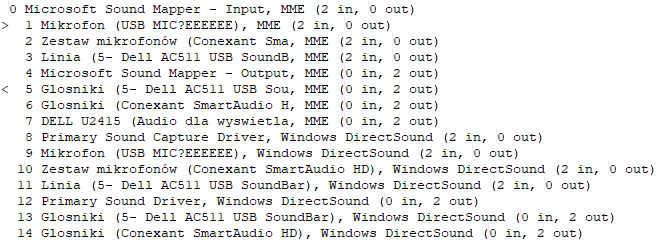
\includegraphics[width=145mm,scale=1.5]{figures/devices.PNG}
    \caption{Spis urządzeń dźwiękowych na maszynie serwera.}
    \label{fig:devices}
    \end{figure}
    
    Rozwiązaniem było automatyczne ustawianie urządzeń na takie jakie w~danym momencie używa system operacyjny.
    \item Nazewnictwo chorób i~powierzchni zęba - w~terminologii stomatologicznej, niektóre obiekty mogą mieć klika nazw. To samo dotyczy się powierzchni zęba. Sprawiało to problemy przy przetwarzaniu komend głosowych. W~celu rozwiązania problemu, stworzono słowniki w~bazie danych. Słownik zawiera zbiór terminów i~ich tłumaczeń. Jeżeli dany obiekt miał kilka nazw, jedna z~nich została wybrana na główną. Reszta nazw jest tłumaczona na nazwę główną. Pozwala to na ujednolicenie interfejsu komunikacji miedzy serwerem, bazą danych i~klientem.
    \item Asynchroniczne przetwarzanie danych - aplikacja klienta wymaga sprawnego przekazywania danych między komponentami aplikacji. Wyzwaniem jest jednak natychmiastowe reagowanie interfejsu graficznego na komendy głosowe lub zmianę wersji danych. Z uwagi na rożne sposoby użytkowania danych, logika klienta jest zaawansowana. Rozwiązano ten problem korzystając z~pełni możliwości technologii Vue, w~temacie działań asynchronicznych. Opis działania technologii można znaleźć w~rozdziale trzecim. 
\end{itemize}

\subsection{Testy}
Aplikacja była testowana po każdej dużej zmianie w~kodzie źródłowym. Testy manualne były przeprowadzane zgodnie z~opisanymi scenariuszami. Scenariusze były rozbudowywane wraz z~aplikacją. Dodatkowo cały system został przetestowany przez pięć osób spoza zespołu deweloperskiego.

Przykładowym punktem scenariusza testowego, był spis komend głosowych. Spis zbudowano w~taki sposób aby zawierał wszystkie słowa zawarte w~bazie danych. Wśród komend były też komendy niepoprawne, w~celu sprawdzenia obsługi błędów użytkownika. Najwięcej testów oraz poprawek dotyczyło interfejsu głosowego. Poniżej przedstawiono zmiany wprowadzone w~systemie komend głosowych, na podstawie testowania aplikacji.
\begin{itemize}
    \item Odmiana słów - każdy użytkownik wypowiada słowa w~unikalny sposób. W~związku z~tym, Google Speech Recognition może nie prawidłowo rozpoznać słowo. Dodatkową trudnością jest nienaturalny ciąg słów w~komendach głosowych np. ,,dwadzieścia jeden sieczna niewyrżnięty''. Z powodu tej nienaturalności system firmy Google może mieć problemy z~użyciem modelu językowego, opisanego w~rozdziale drugim. Efektem może być zrozumienie wspomnianej komendy jako ,,dwadzieścia jeden sieczna niewyrżnięte''. Dla człowieka różnica jest nieznacząca, ale dla komputera jest to inna komenda. W~celu rozwiązania tego problemu zaimplementowano słowniki, o~których budowie wspomniano wcześniej. Dla przykładu, zawartością słownika dla słowa ,,niewyrżnięty'' jest:  ,,niewyrżnięty'', ,,niewyrżnięte'', ,,niewyrżniętych'' i~,,niewyrośnięty''. Wypisane słowa zostały dodane do słownika na podstawie zwróconych przez system słów podczas testów. Analogicznie powstał słownik dla powierzchni zęba. Przykładowo słowa ,,b'', ,,żująca'', ,,żujące'', ,,żując'', ,,sieczna'', ,,sieczny'', ,,sieczne'', ,,siecznych'', oznaczają powierzchnie zęba o~kodzie ,,B''. Kodowanie powierzchni zostało opisane wcześniej w~rozdziale czwartym.
    \item Błąd mikrofonu - uruchomiony interfejs głosowy będzie pobierał komendy w~pętli. W~pierwszej wersji interfejsu głosowego pętla kończyła się po wypowiedzeniu komendy ,,stop''. Problemem była sytuacja, w~której na maszynie serwera nie działał mikrofon. Oznaczało to, że nie dało się zakończyć pętli pobierania komend. Rozwiązaniem było dodanie przycisku dezaktywacji systemu głosowego.
    \item Czas nagrywania komend - system nagrywania oczekuje na pierwszy dźwięk przez dziesięć sekund, następnie każda fraza może trwać do pięć sekund, a~cisza między frazami maksymalnie półtora sekundy. W~pierwszej wersji aplikacji użytkownik nie był informowany kiedy nagrywanie rozpoczyna się i~kończy. Efektem było wypowiadanie dwóch komend podczas jednej sekwencji nagrywania, co kończyło się niepoprawną komendą. Rozwiązano ten problem dodaniem dźwięku startu i~końca nagrywania. Dodano także dźwięk ,,Powtórz komendę.'', w~przypadku podania przez użytkownika błędnej komendy. 
\end{itemize}

Analogicznie na podstawie testów dodano zmiany do warstwy graficznej i~logicznej klienta.

\begin{itemize}
    \item Wielkość grafiki zęba - na diagramie zębów stałych znajdują się aż 32 zębów. Testy wykazały problemy z~wskazaniem myszką w~odpowiednią powierzchnię zęba. Problem rozwiązano za pomocą powiększania zęba. W~momencie najechania myszką na dany ząb, jest on powiększany. Po wykonaniu powtórnie testów zauważono znaczną poprawę w~użytkowaniu diagramu zębowego. Na rysunku \ref{fig:zabPowiekszenie} widać porównanie wielkości przed i~po powiększeniu zęba.
    \begin{figure}[ht!]
    \centering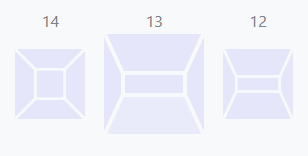
\includegraphics[width=80mm,scale=1.5]{figures/zabPowiekszony.PNG}
    \caption{Porównanie wielkości grafiki zębów przy najechaniu zęba nr 13 wskaźnikiem myszy.}
    \label{fig:zabPowiekszenie}
    \end{figure}
    \item Walidacje pól - na widoku danych osobowych znajduję się wiele pól. Większość z~nich jest opcjonalna. Pola PESEL, imię, nazwisko są obowiązkowe i~podlegają walidacji. Ponieważ jak wykazały testy, użytkownik może zapomnieć uzupełnić numeru PESEL przed zapisem danych. Walidacja numeru PESEL znalazła się także na formatce do wyszukiwania danych pacjentów.
    \item Wersjonowanie - podczas testów zwrócono uwagę na potrzebę przeglądania historii zmian w~diagramach zębowych. Historia zmian rozumiana jest jako historia wizyt pacjenta. W~związku z~tym, dodano proces wersjonowania oraz nowe przyciski na widoku diagramu. Sam proces został dokładnie opisany w~rozdziale czwartym.
\end{itemize}

Poniżej podano przykładowy scenariusz testowy, który użyto do testów.

\begin{enumerate}
    \item W~formatce ,,Podaj pesel'' wprowadź wartość ,,87101912345'', kliknij przycisk ,,Wybierz osobę'' - powinny załadować się dane pacjenta.
    \item Ustaw pole ,,Pesel'' na ,,123'', kliknij ,,Zapisz dane'' - zapis powinien być niemożliwy.
    \item Ustaw pole ,,Pesel'' na ,,87101912345''.
    \item Przejdź na widok diagramu zębów stałych.
    \item Ustaw, klikając myszką, cały ząb o~numerze 14 na ,,Ubytek'' - ząb powinien być cały żółty.
    \item Włącz interfejs głosowy.
    \item Wypowiedz komendę ,,18 bliższa wypełnienie''.
    \item Wypowiedz komendę ,,17 żująca ubytek''.
    \item Wypowiedz komendę ,,46 sieczna próchnica''.
    \item Wypowiedz komendę ,,22 cały most''.
    \item Wypowiedz komendę ,,33 policzkowa ubytek''.
    \item Wypowiedz komendę ,,33 cały usunięty''.
    \item Wypowiedz komendę ,,14 test test'' - system powinien poprosić o~powtórzenie komendy.
    \item Wypowiedz komendę ,,14 cały zdrowy''.
    \item Wypowiedz komendę ,,stop''.
    \item Wróć do widoku danych osobowych i~zapisz dane.
\end{enumerate}
    Podany scenariusz testowy zawiera dodatkowo obraz poprawnego diagramu zębowy. Po przejściu powyższego scenariusza, wygląd diagramu jest zaprezentowany na rysunku \ref{fig:zebyTest}. Dodatkowo programista po każdym przejściu scenariusz sprawdzał poprawność dokumentów na bazie danych, a~także konsole błędów wszystkich komponentów aplikacji.
        \begin{figure}[ht!]
    \centering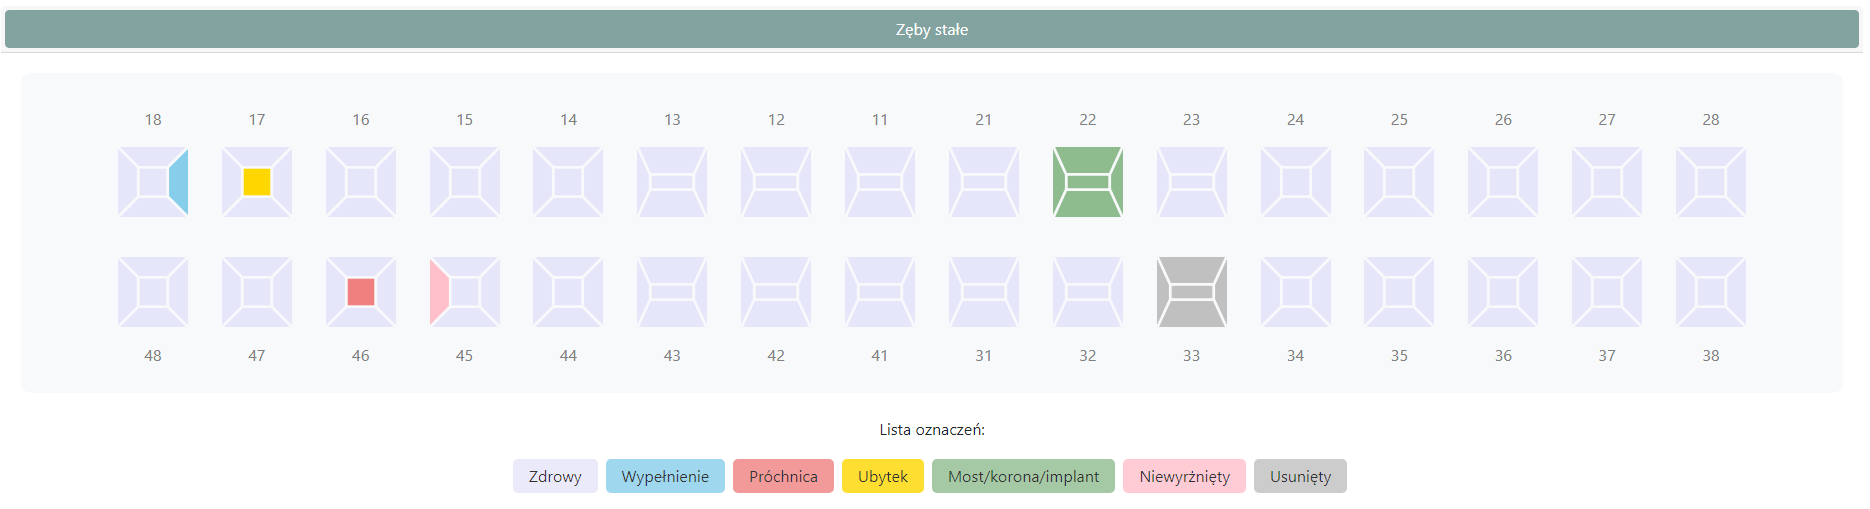
\includegraphics[width=145mm,scale=1.5]{figures/zebyTest.PNG}
    \caption{Poprawny efekt końcowy przykładowego scenariusza testowego.}
    \label{fig:zebyTest}
    \end{figure}

\subsection{Działanie aplikacji}

Aplikacja realizująca moduł diagramu zębowego składa się z dwóch głównych widoków, co zostało opisane w sekcjach wcześniejszych. Pierwszym z nich jest ekran umożliwiający zapis oraz prezentację informacji o pacjencie - jego danych osobowych oraz kontaktowych, drugim - ekran prezentujący diagram zębowy, obrazujący stan uzębienia pacjenta z uwzględnieniem zarówno jego zębów stałych, jak i mlecznych. Poniżej znajduje się dokładny opis wymienionych ekranów.

\subsubsection{Dane osobowe}

Pierwszy widok aplikacji to zakładka \textit{Dane osobowe}. W górnej części umożliwia ona wczytanie wcześniej zapisanych danych. By wyświetlić dane pacjenta, który został już dodany do bazy, należy wprowadzić w wyznaczonym miejscu jego pesel, a następnie zatwierdzić go przyciskiem \textit{Wybierz osobę}. Dane zostaną wówczas wczytane i wyświetlone w formularzu znajdującym się niżej. Forma ta umożliwia jednoczesną prezentację danych z możliwością łatwej ich edycji. Informacjami, które są wymagane, by zapisać dane o pacjencie są pierwsze imię, nazwisko oraz pesel. Sprawdzana jest poprawność tych pól, a efekt walidacji oznaczany jest kolorami zielonym lub czerwonym. Uzupełnienie pozostałych informacji jest opcjonalne i nie uniemożliwia zapisu do bazy danych.

\begin{figure}[ht!]
\centering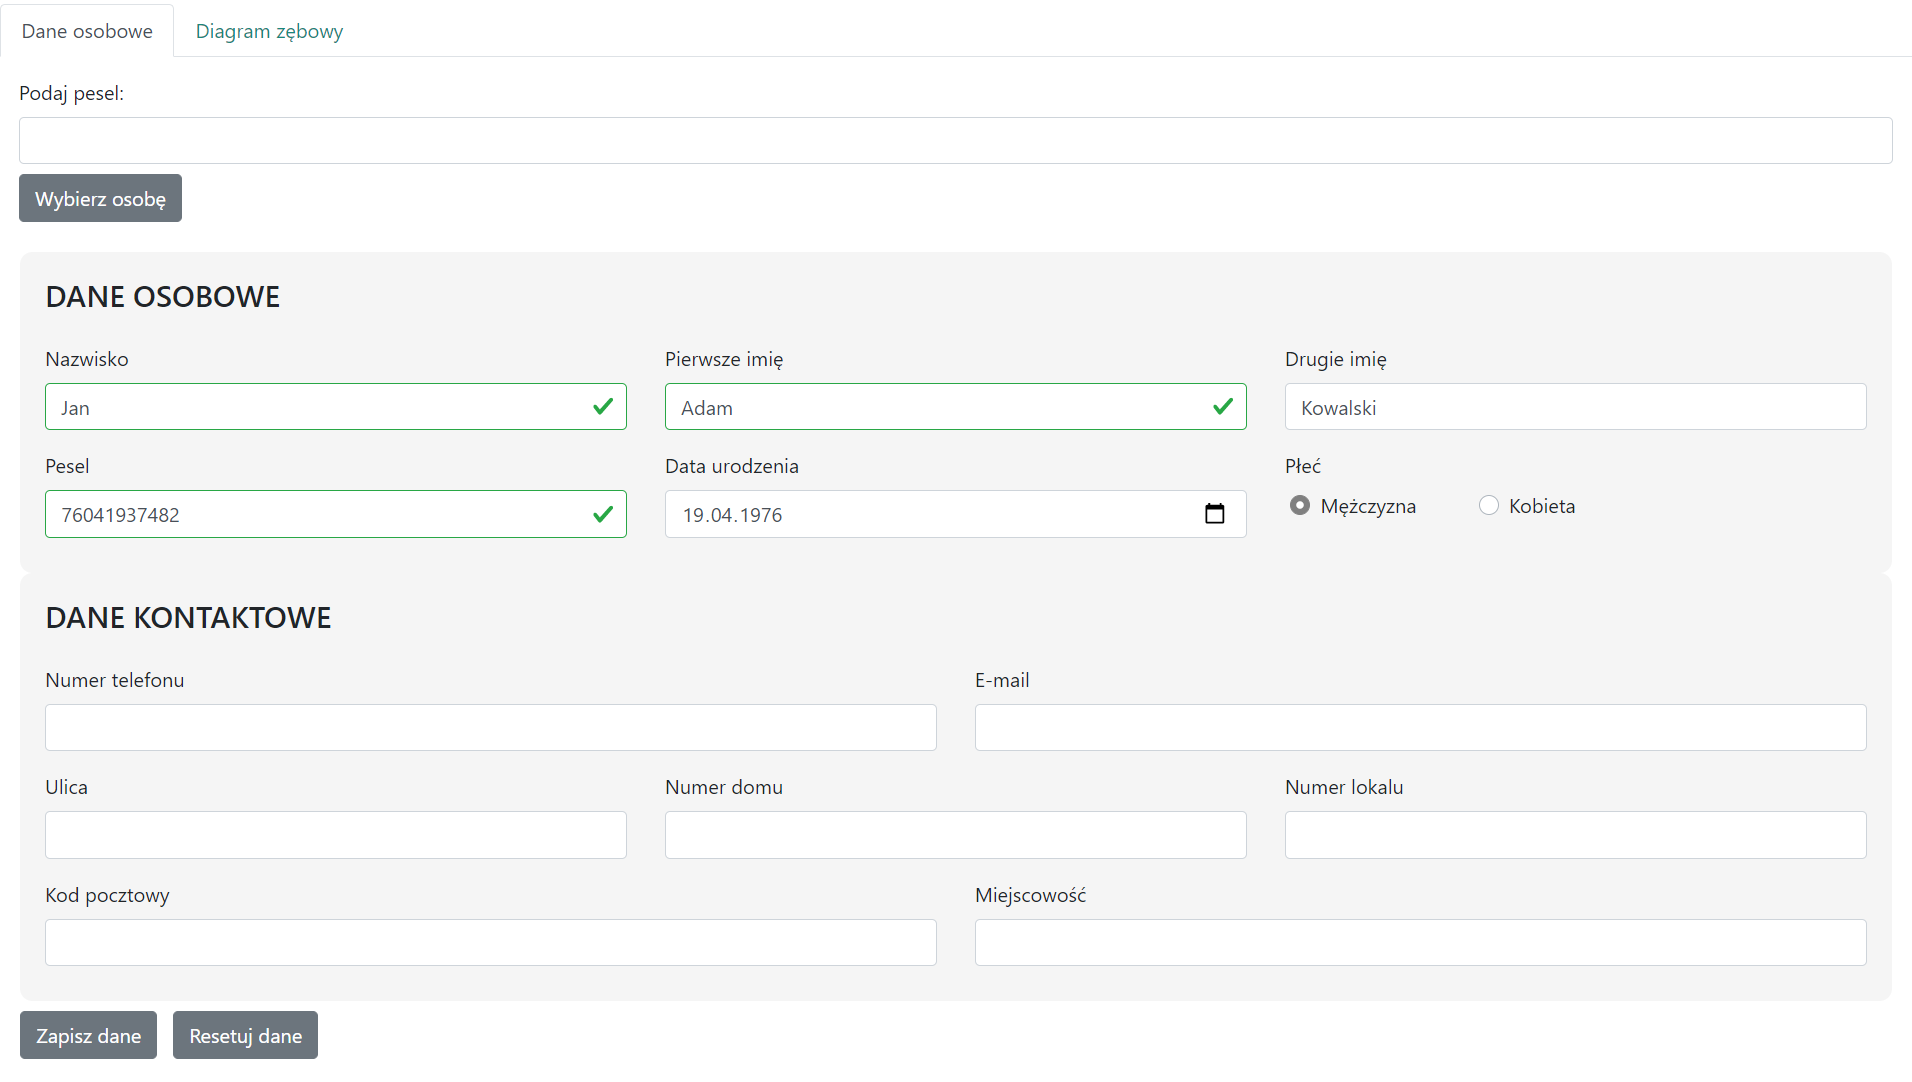
\includegraphics[width=\textwidth]{figures/fromularz.PNG}
\caption{Ekran umożliwiający wprowadzanie do systemu nowych pacjentów oraz przeglądanie i~edycję wcześniej zapisanych danych. \textcolor{red}{błąd!}}
\label{fig:examleForm}
\end{figure}

Widok ten umożliwia także dodanie do bazy nowego pacjenta, którego dane jeszcze się tam nie znajdują. W tym celu należy pominąć pole umożliwiające wprowadzenie szukanego peselu, a jedynie poprawnie uzupełnić prezentowany formularz.

Na dole strony znajdują się dwa przyciski - umożliwiające kolejno zapis lub reset wprowadzonych danych. Po naciśnięciu każdego z nich użytkownik proszony jest o potwierdzenie wybranej operacji. Potwierdzenie zapisu ma zabezpieczyć użytkownika przed utworzeniem zbyt wielu wersji zapisu, gdyż każda z nich jest osobno zapamiętywana w bazie, umożliwiając następnie przegląd tychże wersji. Potwierdzenie resetu ma zapobiec przypadkowemu usunięciu niezapisanych danych. Przycisk ten może zostać wykorzystany w sytuacji, gdy użytkownik chce utworzyć w bazie nowego pacjenta, a wcześniej wczytał inne dane. Po wykonaniu każdej z operacji użytkownik informowany jest o uzyskanym rezultacie. Przykładowe komunikaty zostały pokazane na rysunku \ref{fig:komunikaty}.

\begin{figure}[ht!]
\centering
\includegraphics[width=130mm]{figures/komunikaty.PNG}
\caption{Przykładowe komunikaty prezentowane użytkownikowi}
\label{fig:komunikaty}
\end{figure}

Rysunek \ref{fig:examleForm} przedstawia ekran z przykładowo uzupełnionym formularzem. Uzupełnione zostały wszystkie \textit{Dane osobowe} pacjenta, a dane kontaktowe zostały pominięte. Została sprawdzona poprawność pól wymaganych - \textit{Pierwsze imię}, \textit{Nazwisko} oraz \textit{Pesel} zaznaczone są kolorem zielonym, co oznacza, że mają prawidłowy format. \textit{Data urodzenia} została automatycznie uzupełniona na podstawie podanego peselu.


\subsubsection{Diagram zębowy}

Drugi w kolejności widok, znajdujący się w zakładce \textit{Diagram zębowy}, prezentuje dwa diagramy. Domyślnie wyświetlane są zęby stałe, ale dostępny jest także diagram zębów mlecznych. By ułatwić korzystanie z aplikacji, w górnej części ekranu znajdują się podstawowe dane pacjenta wprowadzone w formularzu. Nad diagramem, po prawej stronie, umieszczone są przyciski umożliwiające przełączanie pomiędzy różnymi wersjami zapisanych danych. Podczas kolejnych wizyt stomatolog lub jego asystent zapisuje dane jako kolejne ich wersje, do których później ma dostęp dzięki wskazanym przyciskom. Wersje oznaczane są datą i godziną. Rysunek \ref{fig:diagram} prezentuje dane zapisane 17 stycznia 2021 roku o godzinie 17:30.

\begin{figure}[ht!]
\centering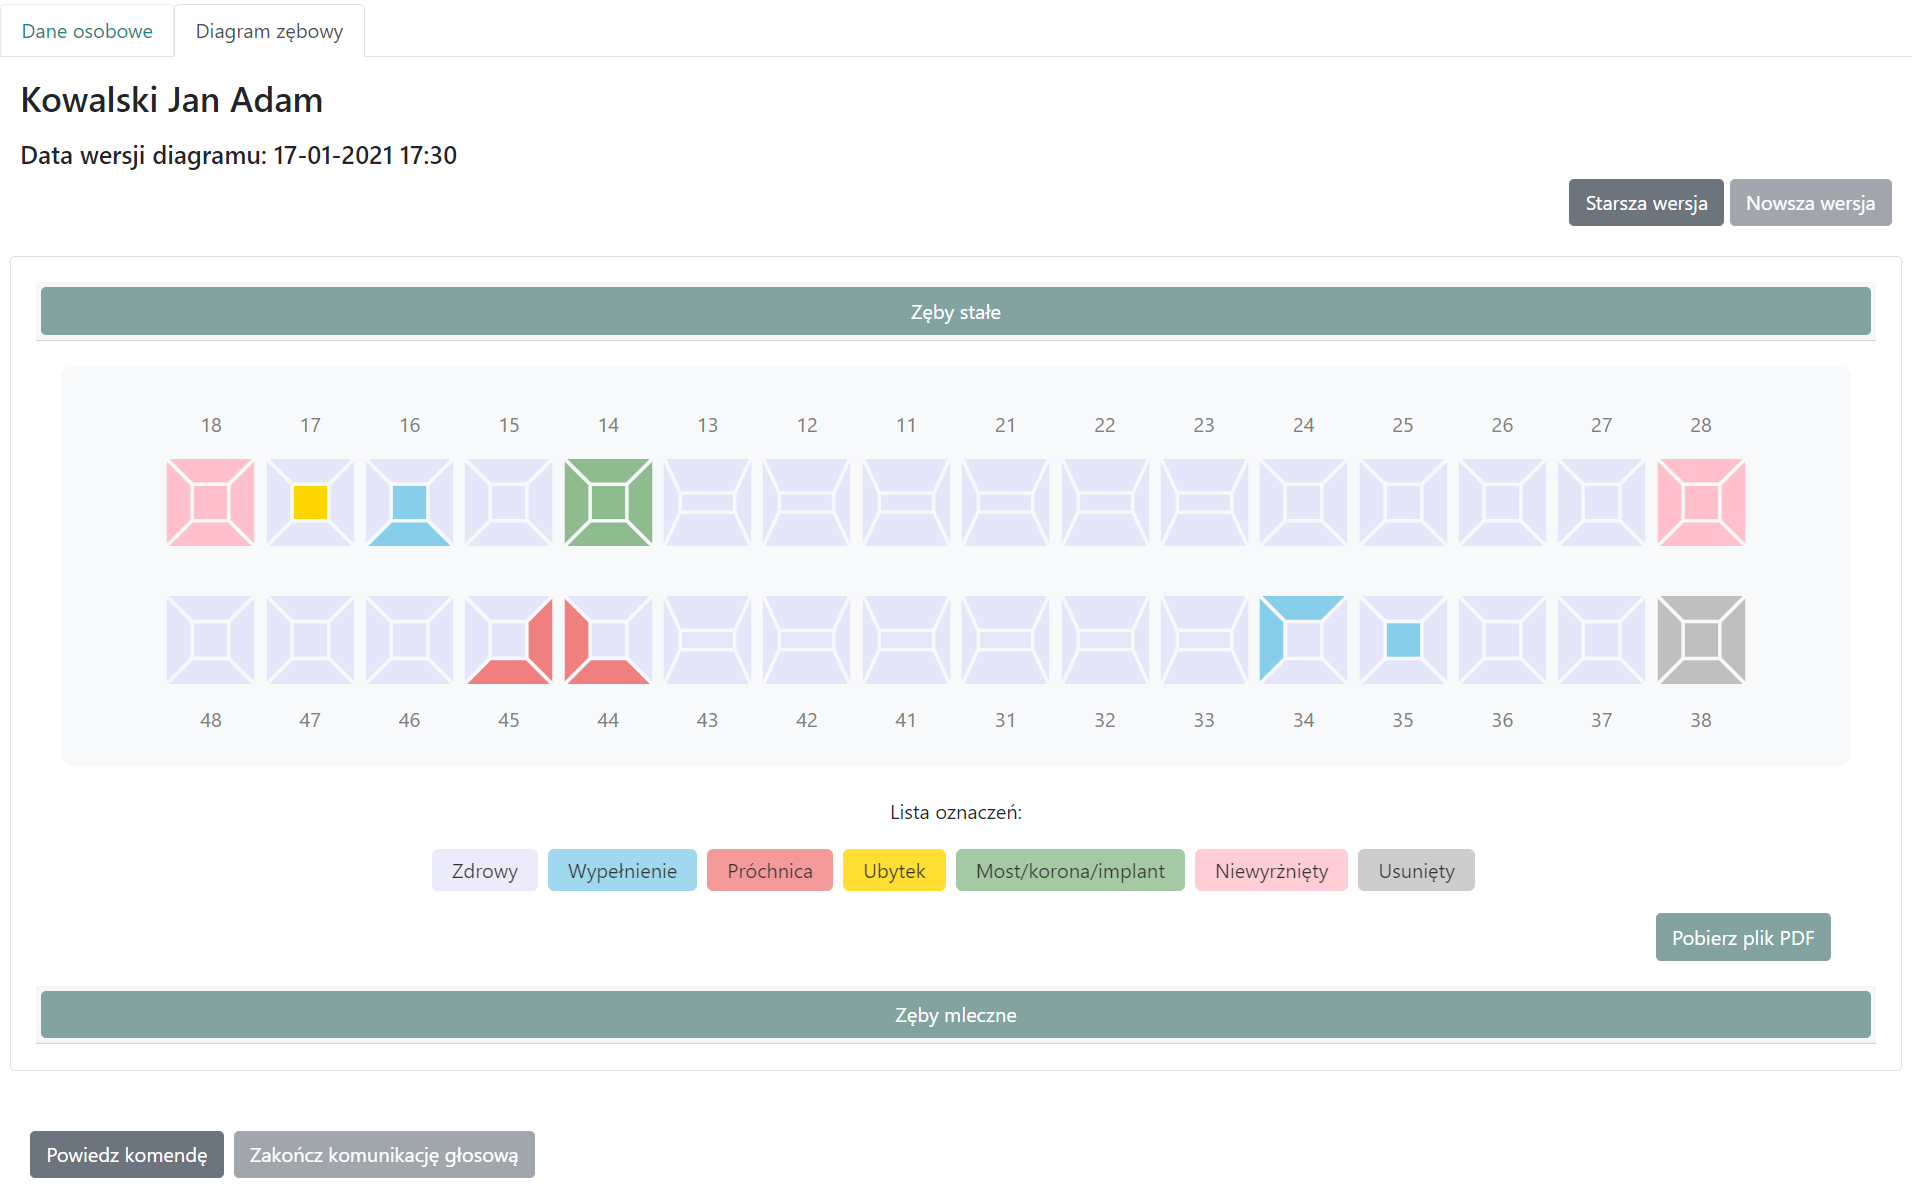
\includegraphics[width=\textwidth]{figures/diagram.PNG}
\caption{Ekran prezentujący diagram zębowy pacjenta}
\label{fig:diagram}
\end{figure}

Głównym elementem drugiego ekranu jest diagram zębowy. Składa się on z trzydziestu dwóch zębów w przypadku diagramu zębów stałych oraz dwudziestu zębów tworzących diagram zębów mlecznych. Użytkownik ma możliwość wybrania zęba, który powiększa się po najechaniu na jego powierzchnię, oraz jednej z pięciu jego części. Kliknięcie wybranego elementu otwiera listę możliwych do wyboru chorób. Po wybraniu jednej z nich część zęba oznaczana jest odpowiednim kolorem. By zwiększyć czytelność diagramu, pod zębami znajduje się lista objaśniająca poszczególne barwy.

Oprócz możliwości wprowadzania danych przy pomocy myszki użytkownik może skorzystać z dostępnego w aplikacji interfejsu głosowego. By aktywować działanie interfejsu trzeba użyć przycisku \textit{Powiedz komendę}, a zakończyć nasłuchiwanie można przyciskiem \textit{Zakończ komunikację głosową} lub wypowiadając komendę \textit{STOP}. Zrozumiane przez system komendy zostają w czasie rzeczywistym nanoszone na diagram. Dodatkowo, w prawym górnym rogu ekranu, w formie komunikatów, wyświetlane są wprowadzane właśnie zmiany. Działanie interfejsu głosowego nie wyklucza możliwości nanoszenia zmian przy użyciu myszki. Obu sposobów można z powodzeniem używać w tym samym czasie. Rysunek \ref{fig:zmiany} pokazuje zmiany wprowadzone na diagramie oraz wyświetlane komunikaty po wypowiedzeniu dwóch komend głosowych - \textit{osiemnaście policzkowa ubytek} oraz \textit{dwadzieścia osiem cały implant}.

\begin{figure}[ht!]
\centering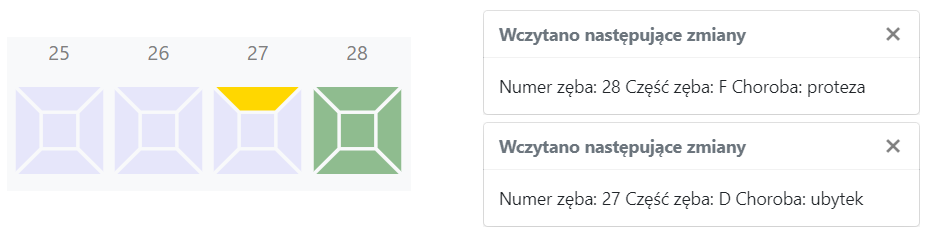
\includegraphics[width=130mm]{figures/zmiany.PNG}
\caption{Przykładowe zmiany wprowadzone przez użytkownika przy pomocy interfejsu głosowego}
\label{fig:zmiany}
\end{figure}

Dodatkowo, by umożliwić przekazywanie danych między pracownikami służby zdrowia, ale także dać możliwość udostępniania danych pacjentom, na ekranie dostępny jest przycisk \textit{Pobierz plik PDF}. Pozwala on na zapis danych do pliku, który można następnie łatwo udostępnić (Rysunek \ref{fig:pdf}).

\begin{figure}[ht!]
\centering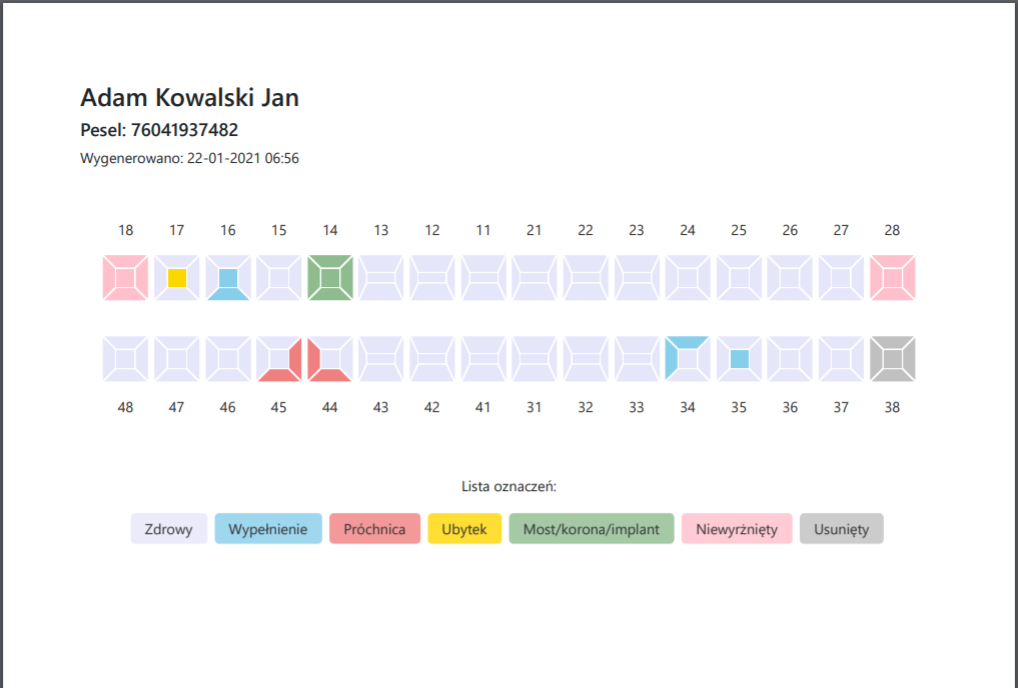
\includegraphics[width=130mm]{figures/pdf.png}
\caption{Fragment wygenerowanego automatycznie pliku PDF.}
\label{fig:pdf}
\end{figure}


\section{Analiza odchylenia toru odwodzenia żuchwy}
\subsection{Wymagania}
W tym module również założono minimalne wymagania produktowe - MVP:
\begin{itemize}
    \item Automatyczne wykrycie górnych i~dolnych zębów
    \item Obliczenie maksymalnego wychylenia żuchwy od stanu początkowego (zaciśniętych zębów) podczas odwodzenia i przywodzenia żuchwy w kątach i milimetrach
    \item Eksportowanie danych do pliku w~formacie pdf
\end{itemize} 
\subsection{Design}
\subsection{Proces instalacji i~uruchomienia}
   \begin{itemize}
    \item zmienić readme w~coś sensownego do czytania :P
    
\end{itemize} 
\subsection{Trudności}
\subsection{Testy}
\subsection{Przykłady użycia}

\chapter{Podsumowanie} 

Rezultatem pracy inżynierskiej są dwa moduły wspomagające analizę i przetwarzanie danych w gabinetach stomatologicznych. Pierwszym modułem jest system oznaczania zębów. Zgodnie z poczynionymi założeniami, system pozwala na:
\begin{itemize}
    \item Utworzenie nowej kartoteki pacjenta lub edycję już istniejącej
    \item Wyświetlanie i edycje danych uzębienia pacjenta za pomocą diagramu zębowego
    \item Wprowadzanie danych do diagramu za pomocą interfejsu głosowego
    \item Eksport diagramu na potrzeby pacjenta
\end{itemize}
Aplikacja pierwszego modułu składa się z klienta i serwera z bazą danych. Klienta można uruchomić za pomocą  najnowszych przeglądarek internetowych. Serwer uruchamiany jest na lokalnej maszynie za pomocą konsoli systemowej.
\newline Drugi moduł dotyczący analizy odchylenia toru odwodzenia żuchwy pozwala na:
\begin{itemize}
    \item Wybranie pliku z lokalnego systemu plików.
    \item Wyświetlenie filmu podczas analizy z zaznaczonymi obliczanymi kątami.
    \item Wyświetlenie maksymalnego odchylenia żuchwy podczas jej odwodzenia w wartościach względnych i bezwzględnych.
    \item Wyświetlenie pełnej analizy w postaci wykresu.
    \item Wybranie fragmentu filmu do analizy.
    \item Zapis wyników, wykresów i zrzutów ekranu w formacie pdf.
\end{itemize}
Tu o exceku ale nie wiem jak to opisać.


Zakończenie pracy zwane również Uwagami końcowymi lub Podsumowaniem powinno zawierać ustosunkowanie
się autora do zadań wskazanych we wstępie do pracy, a w szczególności do celu i zakresu pracy oraz
porównanie ich z faktycznymi wynikami pracy. Podejście takie umożliwia jasne określenie stopnia
realizacji założonych celów oraz zwrócenie uwagi na wyniki osiągnięte przez autora w ramach jego
samodzielnej pracy.

Integralną częścią pracy są również dodatki, aneksy i załączniki zawierające stworzone w ramach pracy programy, aplikacje i projekty.

\section{Rezultaty}
\section{Rozwój i przyszłość}

%--------------------------------------
% Literatura
%--------------------------------------

\bibliographystyle{plain}{\raggedright\sloppy\small\bibliography{bibliografia}}

%--------------------------------------
% Dodatki
%--------------------------------------

%\cleardoublepage\appendix%
%\newpage
%
\chapter{Składanie dokumentu w systemie \LaTeX}

W tym rozdziale znajduje się
garść informacji o tym, jak poprawnie składać tekst pracy w systemie \LaTeX{} wraz z 
przykładami, które mają służyć do przeklejania do własnych dokumentów.

\section{Struktura dokumentu}
\chaptermark{Tytuł rozdziału, jeśli pełen się nie mieści\ldots{}}{}

Praca składa się z rozdziałów (\texttt{chapter}) i podrozdziałów (\texttt{section}).
Ewentualnie można również rozdziały zagnieżdzać (\texttt{subsection}, \texttt{subsubsection}),
jednak nie powinno się wykraczać poza drugi poziom hierarchii (czyli \texttt{subsubsection}).

\section{Akapity i znaki specjalne}

Akapity rozdziela się od siebie przynajmniej jedną pustą linią. Podstawowe
instrukcje, które się przydają to \emph{wyróżnienie pewnych słów}. Można również
stosować \textbf{styl pogrubiony}, choć nie jest to generalnie zalecane.

Należy pamiętać o zasadach polskiej interpunkcji i ortografii. Po spójnikach 
jednoliterowych warto wstawić znak tyldy ($\sim$), który jest tak zwaną
,,twardą spacją'' i powoduje, że wyrazy nią połączone nie będą rozdzielane
na dwie linie tekstu.

Polskie znaki interpunkcyjne różnią się nieco od angielskich: to jest ,,polski'', a to jest
``angielski''. W kodzie źródłowym tego tekstu będzie widać różnicę.

Proszę również zwrócić uwagę na znak myślnika, który może być pauzą ,,---'' lub
półpauzą: ,,--''. Należy stosować je konsekwentnie. Do łączenia wyrazów używamy
zwykłego ,,-'' (\emph{północno-wschodni}), do myślników --- pauzy lub półpauzy.
Inne zasady interpunkcji i typografii można znaleźć w słownikach.

\section{Wypunktowania}

Wypunktowanie z cyframi:
\begin{enumerate}
    \item to jest punkt,
    \item i to jest punkt,
    \item a to jest ostatni punkt.
\end{enumerate}

\noindent
Po wypunktowaniach czasem nie warto wstawiać wcięcia akapitowego. Wtedy przydatne jest
polecenie \texttt{noindent}. Wypunktowanie z kropkami (tzw.~\emph{bullet list}) wygląda tak:
\begin{itemize}
    \item to jest punkt,
    \item i to jest punkt,
    \item a to jest ostatni punkt.
\end{itemize}

\noindent
Wypunktowania opisowe właściwie niewiele się różnią:
\begin{description}
    \item[elementA] to jest opis,
    \item[elementB] i to jest opis,
    \item[elementC] a to jest ostatni opis.
\end{description}


\section{Polecenia pakietu \texttt{ppfcmthesis}}

Parę poleceń zostało zdefiniowanych aby uspójnić styl pracy. Są one przedstawione poniżej
(oczywiście nie trzeba się do nich stosować).

\paragraph{Makra zdefiniowane dla języka angielskiego.} Są nimi: \texttt{termdef} oraz \texttt{acronym}.
Przykłady poniżej obrazują ich przewidywane użycie w tekście.
\begin{center}\footnotesize%
\begin{tabular}{l >{\rightskip\fill}p{12cm}}
\toprule
źródło   & \texttt{we call this a $\backslash$termdef\{Database Management System\} ($\backslash$acronym\{DBMS\})} \\ \cmidrule(lr){2-2}
docelowo & we call this a \termdef{Database Management System} (\acronym{DBMS}) \\ 
\bottomrule
\end{tabular}
\end{center}

\paragraph{Makra zdefiniowane dla języka polskiego.} Podobnie jak dla języka angielskiego zdefiniowano
odpowiedniki polskie: \texttt{defini\-cja}, \texttt{akronim} oraz \texttt{english} dla tłumaczeń angielskich
terminów. Przykłady poniżej obrazują ich przewidywane użycie w tekście.
\begin{center}\footnotesize%
\begin{tabular}{l >{\rightskip\fill}p{12cm}}
\toprule
źródło   & \texttt{nazywamy go $\backslash$definicja\{systemem zarządzania bazą danych\} ($\backslash$akronim\{DBMS\}, $\backslash$english\{Database Management System\})} \\ \cmidrule(lr){2-2}
docelowo & nazywamy go \definicja{systemem zarządzania bazą danych} (\akronim{DBMS}, \english{Database Management System}) \\ \bottomrule
\end{tabular}
\end{center}


\section{Rysunki}

Wszystkie rysunki (w tym również diagramy, szkice i inne) osadzamy w środowisku 
\texttt{figure} i umieszczamy podpis \emph{pod} rysunkiem, w formie elementu \texttt{caption}. Rysunki powinny
zostać umieszczone u góry strony (osadzone bezpośrednio w treści strony zwykle utrudniają czytanie tekstu).
Rysunek~\ref{rys:plama} zawiera przykład pełnego osadzenia rysunku na stronie.

\begin{figure}[t] % możliwe opcje to 't' - top, 'b' - bottom, 'h' - 'here', ale zaleca się 't'
\centering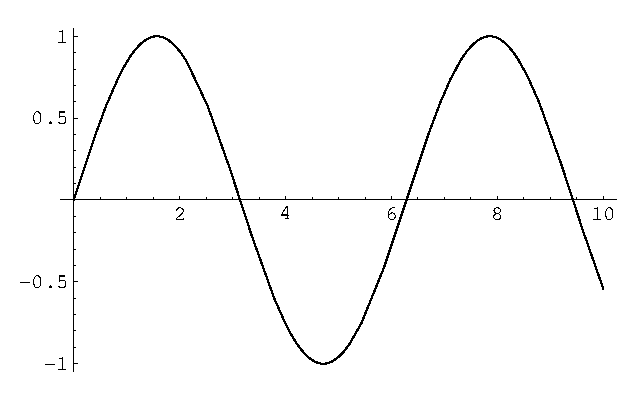
\includegraphics[width=5cm]{figures/mathematica}
\caption{Wykres.}\label{rys:plama}
\end{figure}

\begin{figure}[t]
\centering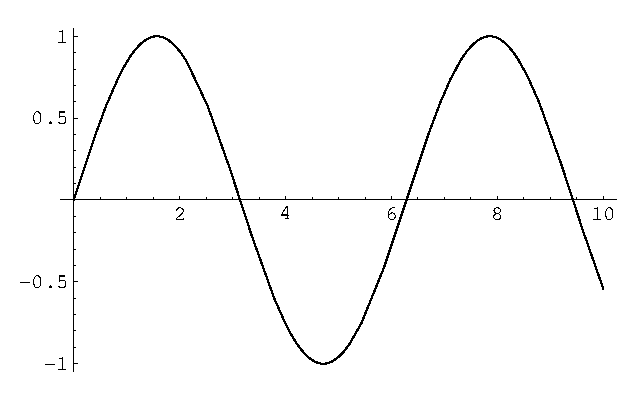
\includegraphics[width=\textwidth]{figures/mathematica}
\fcmfcaption{Ten sam wykres ale na szerokość tekstu. Formatowanie podpisu zgodne z wytycznymi FCMu.}\label{rys:plama2}
\end{figure}

Styl FCMu to nieco inne nagłówki rysunków. Dostepne są one poleceniem \texttt{fcmfcaption} (zob.~rysunek
\ref{rys:plama2}).

\subsection{Tablice}

Tablice to piękna rzecz, choć akurat ich umiejętne tworzenie w \LaTeX{}u nie jest łatwe. 
Jeśli tablica jest skomplikowana, to można ją na przykład wykonać w programie
OpenOffice, a następnie wyeksportować jako plik \akronim{PDF}. W każdym przypadku tablice wstawia się podobnie
jak rysunki, tylko że w środowisko \texttt{table}. Tradycja typograficzna sugeruje umieszczenie opisu tablicy, a więc
elementu \texttt{caption} ponad jej treścią (inaczej niż przy rysunkach).  

Tablica~\ref{tab:tabela} pokazuje pełen przykład.

\begin{table}[ht]
\caption{Przykładowa tabela. Styl opisu jest zgodny z rysunkami.}\label{tab:tabela}
\centering\footnotesize%
\begin{tabular}{l c}
\toprule
artykuł & cena [zł] \\
\midrule
bułka   & $0,4$ \\
masło   & $2,5$ \\
\bottomrule
\end{tabular}
\end{table}

Zasady FCMu sugerują nieco inne nagłówki tablic. Dostepne są one poleceniem \texttt{fcmtcaption} (zob.~tablicę
\ref{tab:tabela2}).

\begin{table}[ht]
\fcmtcaption{Przykładowa tabela. Styl opisu jest zgodny z wytycznymi FCMu.}\label{tab:tabela2}
\centering\footnotesize%
\begin{tabular}{l c}
\toprule
artykuł & cena [zł] \\
\midrule
bułka   & $0,4$ \\
masło   & $2,5$ \\
\bottomrule
\end{tabular}
\end{table}


\subsection{Checklista}

\begin{itemize}
\item Znakiem myślnika jest w LaTeXu dywiz pełen (---) albo półpauza (--), przykład:
  A niech to jasna cholera --- wrzasnąłem.

\item Połączenie między wyrazami to zwykły myślnik, przykład:   północno-zachodni

\item Sprawdź czy tutuł pracy ma maksymalnie dwa wiersze i czy stanowią one pełne frazy
  (czy nie ma przeniesienia bez sensu).

\item Sprawdź ostrzeżenia o 'overfull' i 'underful' boxes. Niektóre z nich można zignorować (spójrz
  na wynik formatowania), niektóre trzeba poprawić; czasem przeformułować zdanie.

item Przypisy stawia się wewnątrz zdań lub za kropką, przykład:
  Footnote is added after a comma.\footnote{Here is a footnote.}

\item Nie używaj przypisów zbyt często. Zobacz, czy nie lepiej będzie zintegrować przypis z tekstem.

\item Tytuły tabel, rysunków powinny kończyć się kropką.

\item Nie używaj modyfikatora [h] (here) do rysunków i tabel. Rysunki i tabele powinny być
  justowane do góry strony lub na stronie osobnej.

\item Wyróżnienie w tekście to polecenie \emph{wyraz}, nie należy używać czcionki pogrubionej (która
  wystaje wizualnie z tekstu i rozprasza).

\item Nazwy plików, katalogów, ścieżek, zmiennych środowiskowych, klas i metod formatujemy poleceniem
  \texttt{plik\_o\_pewnej\_nazwie}.

\item Po ostatniej zmianie do treści, sprawdź i przenieś wiszące spójniki wstawiając przed nie znak
  tyldy (twardej spacji), przykład:
  Ala i~kotek nie lubią mleczka, a~Stasiu lubi.
  
\item Za i.e. (id est) i e.g. (exempli gratia) stawia się zwyczajowo przecinek w typografii amerykańskiej.

\item Przed i za pełną pauza nie ma zwyczajowo spacji w typografii amerykańskiej, przykład:
  Darn, this looks good---said Mary.

\item Zamykający cudzysłów oraz footnote wychodzą za ostatni znak interpunkcji w typografii 
  amerykańskiej, przykłady:
  It can be called a ``curiosity,'' but it's actually normal.
  Footnote is added after a comma.\footnote{Here is a footnote.}

\item Odwołania do tabel i rysunków zawsze z wielkiej litery, przykład:
  In Figure~\ref{rys:plama} we illustrated XXX and in Table~\ref{tab:tabela} we show detailed data.
  
\end{itemize}


\section{Literatura i materiały dodatkowe}

Materiałów jest mnóstwo. Oto parę z nich:
\begin{itemize}
    \item \emph{The Not So Short Introduction\ldots}, która posiada również tłumaczenie 
    w języku polskim.\\
    \url{http://www.ctan.org/tex-archive/info/lshort/english/lshort.pdf}

    \item Klasy stylu \texttt{memoir} posiadają bardzo wiele informacji o składzie tekstów
    anglosaskich oraz sposoby dostosowania \LaTeX{}a do własnych potrzeb.\\
    \url{http://www.ctan.org/tex-archive/macros/latex/contrib/memoir/memman.pdf}
    
    \item Nasza grupa dyskusyjna i repozytorium Git są również dobrym miejscem aby zapytać
    (lub sprawdzić czy pytanie nie zostało już zadane).\\
    \url{https://github.com/politechnika/put-latex}

    \item Dla łaknących więcej wiedzy o systemie LaTeX podstawowym źródłem informacji
    jest książka Lamporta~\cite{Lamport1985}. Prawdziwy \emph{hardcore} to oczywiście
    \emph{The \TeX{}book} profesora Knutha~\cite{Knuth1986}.
\end{itemize}



%--------------------------------------
% Informacja o prawach autorskich
%--------------------------------------

\ppcolophon

\end{document}
